\chapter{Implementación del Proyecto}
\label{chap:planificacion}


%   \section{Análisis}
%   \label{sec:Analisis}
% %
%     % La programación extrema no contempla específicamente el diseño de casos de uso
%     Dentro del análisis se realizó el diseño de Casos de Uso como parte del proceso para entender el comportamiento del sistema. \cite{casos_uso}
% %
%
% \begin{figure}[H]
%   \begin{center}
%     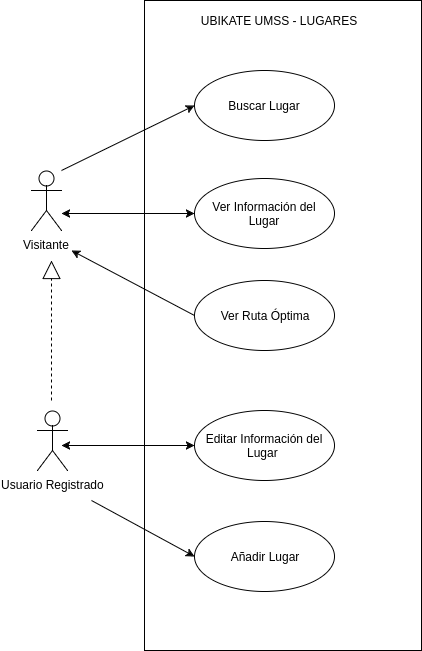
\includegraphics[width=0.45\textwidth]{casos_uso/cu_lugares}
%   \end{center}
%   \caption{Diagrama Casos de Uso - Gestion de Lugares }
%   \label{fig:cu_lugares}
%   \caption*{Fuente: Elaboración propia}
% \end{figure}
%
% \begin{table}[H]
  \begin{center}
    \begin{tabularx}{0.75\textwidth}{ X X  }
      \toprule
      \multicolumn{2}{l}{\textbf{Caso de Uso:} Buscar Lugar} \\
      \multicolumn{2}{l}{\textbf{Actor:} Visitante} \\
      \multicolumn{2}{l}{\textbf{Precondición:} El Visitante accede al sistema.} \\
      \addlinespace
      \textbf{Secuencia Principal} & \textbf{Alternativas} \\
      \midrule
      1. El Visitante accede a la sección de ``Lugares''. \\
      \addlinespace
      2. El visitante ingresa el nombre del lugar en un \emph{search box}.  \\
      \addlinespace
      3. El Visitante ve la lista de Lugares registrados que coinciden con la búsqueda. &
      3.1 El lugar no existe en la base de datos, retorna una lista vacía. \\

      \midrule
      \multicolumn{2}{l}{\textbf{Postcondición:} El Visitante encuentra un lugar} \\

      \bottomrule
    \end{tabularx}
    \caption{Caso de Uso - Buscar Lugar}
    \label{tab:cu_buscar_lugar}
  \end{center}
\end{table}


% \begin{table}[H]
%   \begin{center}
%     \begin{tabularx}{0.75\textwidth}{  L{3cm} X  }
%       \toprule
%       \textbf{Caso de Uso:} & Buscar Lugar \\
%       \textbf{Actor:} & Visitante \\
%       \textbf{Precondición:} & El Visitante accede al sistema. \\
%       \textbf{Secuencia Principal:} & 1. El Visitante accede a la sección de ``Lugares''. \\
%       \addlinespace
%       & 2. El visitante ingresa el nombre del lugar en un \emph{search box}.  \\
%       \addlinespace
%       & 3. El Visitante ve la lista de Lugares registrados que coinciden con la búsqueda. \\
%
%       \addlinespace
%       \textbf{Postcondición:} & El Visitante encuentra un lugar. \\
%       \bottomrule
%     \end{tabularx}
%     \caption{Caso de Uso - Buscar Lugar}
%     \label{tab:cu_buscar_lugar}
%   \end{center}
% \end{table}




\begin{table}[H]
  \begin{center}
    \begin{tabularx}{0.75\textwidth}{ X X  }
      \toprule
      \multicolumn{2}{l}{\textbf{Caso de Uso:} Ver Información del Lugar} \\
      \multicolumn{2}{l}{\textbf{Actor:} Visitante} \\
      \multicolumn{2}{l}{\textbf{Precondición:} El Visitante ha buscado un lugar} \\
      \addlinespace
      \textbf{Secuencia Principal} & \textbf{Alternativas} \\
      \midrule
      1. El Visitante hace un tap sobre el nombre del lugar en la lista de búsqueda. \\
      \addlinespace
      2. El visitante puede ver una imagen del lugar. &
      2.1. Si el lugar no tiene una imagen asociada, se desplegará una imagen genérica de la UMSS.\\
      \addlinespace
      3. El Visitante ve la descripción del lugar. & \\

      \midrule
      \multicolumn{2}{l}{\textbf{Postcondición:} El Visitante puede ver la información del lugar.} \\
      \bottomrule
    \end{tabularx}
    \caption{Caso de Uso - Ver Información del lugar}
    \label{tab:cu_info_lugar}
  \end{center}
\end{table}


\begin{table}[H]
  \begin{center}
    \begin{tabularx}{0.75\textwidth}{ X X  }
      \toprule
      \multicolumn{2}{l}{\textbf{Caso de Uso:} Ver Ruta Óptima} \\
      \multicolumn{2}{l}{\textbf{Actor:} Visitante} \\
      \multicolumn{2}{l}{\textbf{Precondición:} El Visitante observa la información del lugar.} \\
      \addlinespace
      \textbf{Secuencia Principal} & \textbf{Alternativas} \\
      \midrule
      1. El Visitante selecciona el botón que muestra la ruta más corta al lugar. & \\
      \addlinespace
      2. El sistema pregunta si el usuario quiere compartir su ubicación geográfica. & \\
      \addlinespace
      3. El Visitante acepta la pregunta. &
      3.1. Si el usuario niega la pregunta, el sistema no puede mostrar la ruta óptima. \\

      \midrule
      \multicolumn{2}{L{11cm}}{\textbf{Postcondición:} El Visitante ve un mapa con un marcador y una línea mostrando la ruta óptima. } \\

      \bottomrule
    \end{tabularx}
    \caption{Caso de Uso - Ver Ruta Óptima}
    \label{tab:cu_ruta_optima}
  \end{center}
\end{table}




% \begin{table}[H]
%   \begin{center}
%     \begin{tabularx}{0.75\textwidth}{ X X  }
%       \toprule
%       \multicolumn{2}{l}{\textbf{Caso de Uso:} Ver Ruta Óptima} \\
%       \multicolumn{2}{l}{\textbf{Actor:} Visitante} \\
%       \multicolumn{2}{l}{\textbf{Precondición:} El Visitante está viendo la información del lugar.} \\
%       \addlinespace
%       \textbf{Secuencia Principal} & \textbf{Alternativas} \\
%       \midrule
%       1. El Visitante selecciona el botón que muestra la ruta más corta al lugar. & \\
%       \addlinespace
%       2. El sistema pregunta si el usuario quiere compartir su ubicación geográfica. & \\
%       \addlinespace
%       3. El Visitante acepta la pregunta. &
%       3.1. Si el usuario niega la pregunta, el sistema no puede mostrar la ruta óptima.\\
%
%       \midrule
%       \multicolumn{2}{l}{\textbf{Postcondición:} El Visitante ve un mapa con el lugar marcado y una línea que conecta la posición actual del usuario con el lugar.} \\
%
%       \bottomrule
%     \end{tabularx}
%     \caption{Caso de Uso - Ver Ruta Óptima}
%     \label{tab:cu_ruta_optima}
%   \end{center}
% \end{table}
%
%



\begin{table}[H]
  \begin{center}
    \begin{tabularx}{0.75\textwidth}{ X X  }
      \toprule
      \multicolumn{2}{l}{\textbf{Caso de Uso:} Editar Información del Lugar} \\
      \multicolumn{2}{l}{\textbf{Actor:} Visitante Registrado} \\
      \multicolumn{2}{L{12cm}}{\textbf{Precondición:} El Visitante Registrado esta viendo la información del lugar.} \\
      \addlinespace
      \textbf{Secuencia Principal} & \textbf{Alternativas} \\
      \midrule
      1. El Visitante Registrado selecciona el boton de Edicion. \\
      \addlinespace
      2. El sistema muestra un formulario con la información actual del Lugar.& \\
      \addlinespace
      3. El Visitante Registrado selecciona el botón ``Aceptar''. & \\


      \midrule
      \multicolumn{2}{L{11cm}}{\textbf{Postcondición:} El sistema muestra la información del Lugar actualizada.} \\

      \bottomrule
    \end{tabularx}
    \caption{Caso de Uso - Editar Información del Lugar}
    \label{tab:cu_edit_place}
  \end{center}
\end{table}


\begin{table}[H]
  \begin{center}
    \begin{tabularx}{0.75\textwidth}{ X X }
      \toprule
      \multicolumn{2}{l}{\textbf{Caso de Uso:} Añadir Lugar} \\
      \multicolumn{2}{l}{\textbf{Actor:} Visitante Registrado} \\
      \multicolumn{2}{L{12cm}}{\textbf{Precondición:} El Visitante Registrado necesita desplazarse hasta el lugar para añadirlo.} \\
      \addlinespace
      \textbf{Secuencia Principal} & \textbf{Alternativas} \\
      \midrule
      1. El Visitante Registrado ha accedido a la sección de ``Lugares''. & \\
      \addlinespace
      2. El Visitante Registrado puede ver un botón de adición al final de la lista de lugares. &\\
      \addlinespace
      3. El sistema pregunta si se desea compartir la ubicación geográfica.
      \addlinespace
      3. El Visitante Registrado acepta la pregunta. &
      3.1. El visitante niega la pregunta.\\
      \addlinespace
      4. El Visitante Registrado ve un formulario para ingresar la información del lugar. &
      4.1. El Visitante Registrado no puede anadir un nuevo lugar. \\
      \addlinespace
      5. El Visitante Registrado acepta el formulario. & \\

      \midrule
      \multicolumn{2}{l}{\textbf{Postcondición:} El sistema muestra el lugar en la lista de lugares.} \\

      \bottomrule
    \end{tabularx}
    \caption{Caso de Uso - Añadir Lugar}
    \label{tab:cu_add_place}
  \end{center}
\end{table}

%
% \begin{figure}[H]
%   \begin{center}
%     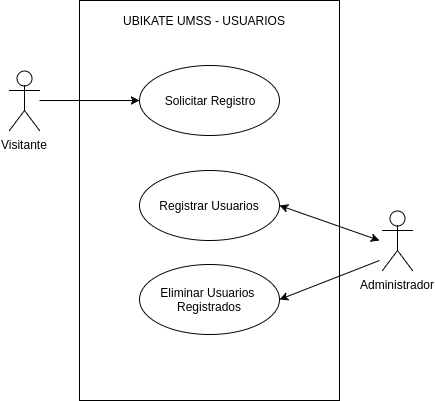
\includegraphics[width=0.45\textwidth]{casos_uso/cu_usuarios}
%   \end{center}
%   \caption{Diagrama Casos de Uso - Gestion de Usuarios }
%   \label{fig:cu_usuarios}
%   \caption*{Fuente: Elaboración propia}
% \end{figure}
%
% \begin{table}[H]
  \begin{center}
    \begin{tabularx}{0.75\textwidth}{ X X  }
      \toprule
      \multicolumn{2}{l}{\textbf{Caso de Uso:} Solicitar Registro} \\
      \multicolumn{2}{l}{\textbf{Actor:} Visitante} \\
      \multicolumn{2}{l}{\textbf{Precondición:} El Visitante accede al sistema.} \\
      \addlinespace
      \textbf{Secuencia Principal} & \textbf{Alternativas} \\
      \midrule
      1. El Visitante accede a la sección de ``Registro''. \\
      \addlinespace
      2. El visitante ingresa su nombre y una direccion email.  \\

      \midrule
      \multicolumn{2}{l}{\textbf{Postcondición:} El Visitante ve un mensaje de confirmacion} \\

      \bottomrule
    \end{tabularx}
    \caption{Caso de Uso - Solicitar Registro}
    \label{tab:cu_solicitar_registro}
  \end{center}
\end{table}


\begin{table}[H]
  \begin{center}
    \begin{tabularx}{0.75\textwidth}{ X X  }
      \toprule
      \multicolumn{2}{l}{\textbf{Caso de Uso:} Registrar Usuario} \\
      \multicolumn{2}{l}{\textbf{Actor:} Administrador} \\
      \multicolumn{2}{l}{\textbf{Precondición:} El Administrador accede al sistema.} \\
      \addlinespace
      \textbf{Secuencia Principal} & \textbf{Alternativas} \\
      \midrule
      1. El Administrador accede a la sección de ``Registro de Usuarios''. \\
      \addlinespace
      2. El Administrador ve una lista con de usuarios a registrar.  \\
      \addlinespace
      3. El Administrador acepta el registro del usuario.  \\
      \addlinespace
      3. El sistema manda un email con instrucciones al usuario.  \\
      \addlinespace
      4. Un mensaje confirmando el envio del email es mostrado. & 4.1. Si el email no existe, un mensaje es mostrado y el registro del usuario es cancelado.  \\

      \midrule
      \multicolumn{2}{L{12cm}}{\textbf{Postcondición:} El Visitante deberia recibir un email con instrucciones de registro.} \\

      \bottomrule
    \end{tabularx}
    \caption{Caso de Uso - Registrar Usuario}
    \label{tab:cu_solicitar_registro}
  \end{center}
\end{table}



\begin{table}[H]
  \begin{center}
    \begin{tabularx}{0.75\textwidth}{ X X  }
      \toprule
      \multicolumn{2}{l}{\textbf{Caso de Uso:} Eliminar Usuarios Registrados} \\
      \multicolumn{2}{l}{\textbf{Actor:} Administrador} \\
      \multicolumn{2}{l}{\textbf{Precondición:} El Administrador accede al sistema.} \\
      \addlinespace
      \textbf{Secuencia Principal} & \textbf{Alternativas} \\
      \midrule
      1. El Administrador accede a la sección de ``Usuarios Registrados''. \\
      \addlinespace
      2. El Administrador elimina un usuario registrado.  \\
      \addlinespace
      3. Un mensaje confirmando la eliminacion del usuario es mostrado.\\

      \midrule
      \multicolumn{2}{L{11.5cm}}{\textbf{Postcondición:} El Usuario eliminado ya no deberia ser visible en la lista de Usuarios registrados.} \\

      \bottomrule
    \end{tabularx}
    \caption{Caso de Uso - Eliminar Usuarios Registrados}
    \label{tab:cu_solicitar_registro}
  \end{center}
\end{table}

%
%
% \begin{figure}[H]
%   \begin{center}
%     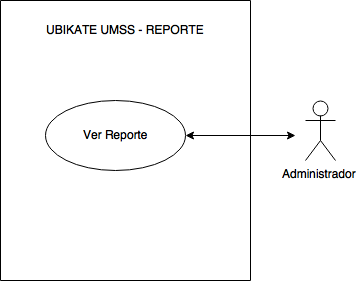
\includegraphics[width=0.45\textwidth]{casos_uso/cu_reporte}
%   \end{center}
%   \caption{Diagrama Casos de Uso - Reporte }
%   \label{fig:cu_reporte}
%   \caption*{Fuente: Elaboración propia}
% \end{figure}
%
% \begin{table}[H]
  \begin{center}
    \begin{tabularx}{0.75\textwidth}{ X X  }
      \toprule
      \multicolumn{2}{l}{\textbf{Caso de Uso:} Ver Reporte} \\
      \multicolumn{2}{l}{\textbf{Actor:} Administrador} \\
      \multicolumn{2}{l}{\textbf{Precondición:} El Administrador accede al sistema.} \\
      \addlinespace
      \textbf{Secuencia Principal} & \textbf{Alternativas} \\
      \midrule
      1. El Administrador accede a la sección de ``Reporte''. \\
      \addlinespace
      2. El Sistema genera una grafica en relacion a los lugares mas visitados.  \\

      % \midrule
      % \multicolumn{2}{l}{\textbf{Postcondición:} El Visitante encuentra un lugar} \\

      \bottomrule
    \end{tabularx}
    \caption{Caso de Uso - Ver Reporte}
    \label{tab:cu_ver_reporte}
  \end{center}
\end{table}



% Siguiendo la metodología XP, el presente proyecto de grado debe empezar por la primera etapa del Planning Game.\\


% Exploración - Entrega y estimación de las historias de usuario


\section{Exploración}
\label{sec:requerimientos}


Como parte del proceso de Exploración se empezó identificando los usuarios que tomarán parte del sistema y los requerimientos funcionales que el sistema deberá proveer, para posteriormente definir las \emph{historias de usuario}.

% Como parte del analisis, se procedió a elaborar la lista de requerimientos funcionales y no-funcionales, los requerimientos funcionales vienen a ser las características o servicios que el sistema proveerá a sus usuarios y los requerimientos no funcionales son las propiedades o restricciones del sistema.

\subsection{Identificación de Usuarios}

Se puede identificar 3 tipos de usuario en el sistema:

\begin{itemize}

\item \textbf{Usuario Visitante:} Un usuario visitante puede ver los lugares que están registrados en el sistema, su información y la ruta óptima al lugar.

\item \textbf{Usuario Registrado:} Un usuario registrado tiene privilegios para agregar lugares y poder editarlos según se requiera.

\item \textbf{Usuario Administrador:} Un administrador tiene privilegios para remover usuarios registrados que estén haciendo uso indebido del sistema y además pueden ver los reportes que el sistema ofrezca.

\end{itemize}


\subsection{Requerimientos Funcionales}

\LTXtable{0.75\textwidth}{implementacion/requerimientos_funcionales}

% \subsection{Requerimientos No Funcionales}
%
% \LTXtable{0.75\textwidth}{implementacion/requerimientos_no_funcionales}




  \subsection{Historias de Usuario}
  \label{sub:historias_de_usuario}

    Las \emph{Historias de Usuario}, descritas a continuacion, están escritas en lenguaje del cliente (no técnico) y serán la pauta para  determinar que los requerimientos del sistema están correctamente implementados.

    % % % user_story_01
% % \begin{table}[!ht]
% \begin{table}[H]
%   \begin{center}
%     \begin{tabular}{ L{3cm}  L{8cm} }
%       \toprule
%         \textbf{Historia} US01 &
%         % \textbf{Esfuerzo} 5 puntos \\
%         \makebox[6cm][r]{\textbf{Esfuerzo} 8 puntos} \\
%         % \makebox[4cm][r]{\textbf{Estimación} 3 días} \\
%
%       \midrule
%       \multirow{3}{*}{\textbf{Descripción}}
%         & Yo como visitante\\
%         & Deseo registrarme en el sistema\\
%         & Para poder acceder al sistema\\
%       \midrule
%         \multirow{3}{3cm}{\textbf{Criterios de Aceptación}}
%         & Quiero ver fácilmente que no estoy registrado\\
%         & Quiero que el registro solamente me pida un nombre de usuario y un password\\
%         & Quiero ver que al estar registrado pueda acceder a los lugares\\
%       \bottomrule
%     \end{tabular}
%     \caption{Historia de Usuario - US01}
%     \label{tab:user_story_01}
%   \end{center}
% \end{table}

% user_story_02

% user_story_03

\begin{table}[H]
  \begin{center}
    \begin{tabular}{ L{3cm}  L{8cm} }
      \toprule
        \textbf{Código:} & US01 \\
        \textbf{Prioridad:} & Alta \\
        \textbf{Riesgo:} & Alta \\

        % \addlinespace
      \midrule
        \multirow{3}{*}{\textbf{Descripción:}}
        & Yo como visitante\\
        & Deseo ver una lista de lugares \\
        % & Deseo ingresar el nombre de un lugar\\
        & Para encontrar el lugar al que deseo ir\\
        \addlinespace
      % \midrule
        \multirow{3}{3cm}{\textbf{Criterios de Aceptación:}}
        & Quiero tener los lugares en una base de datos \\
        & Quiero ver una lista de lugares\\
        & Quiero filtrar la lista de lugares por el nombre o parte de este\\
        % & Quiero encontrar un lugar
        % & Quiero encontrar un lugar y poder ver su información\\
      \bottomrule
    \end{tabular}
    \caption{Historia de Usuario - US01}
    \label{tab:user_story_01}
  \end{center}
\end{table}

\begin{table}[H]
  \begin{center}
    \begin{tabular}{ L{3cm}  L{8cm} }
      \toprule
        \textbf{Historia} US02 &
        % \textbf{Esfuerzo} 5 puntos \\
        \makebox[6cm][r]{\textbf{Esfuerzo} 8 puntos} \\
        % \makebox[4cm][r]{\textbf{Estimación} 3 días} \\

      \midrule
        \multirow{3}{*}{\textbf{Descripción}}
        & Yo como visitante\\
        & Deseo ver la información de un lugar\\
        & Para decidir si es el lugar que estoy buscando\\
      \midrule
        \multirow{3}{3cm}{\textbf{Criterios de Aceptación}}
        & Quiero leer una descripción del lugar\\
        & Quiero ver un teléfono asociado al lugar\\
        & Quiero ver en qué piso se encuentra el lugar\\
      \bottomrule
    \end{tabular}
    \caption{Historia de Usuario - US02}
    \label{tab:user_story_02}
  \end{center}
\end{table}



% user_story_03

\begin{table}[H]
  \begin{center}
    \begin{tabular}{ L{3cm}  L{8cm} }
      \toprule
        \textbf{Historia} US03 &
        % \textbf{Esfuerzo} 5 puntos \\
        \makebox[6cm][r]{\textbf{Esfuerzo} 8 puntos} \\
        % \makebox[4cm][r]{\textbf{Estimación} 3 días} \\

      \midrule
        \multirow{3}{*}{\textbf{Descripción}}
        & Yo como visitante\\
        & Deseo ver el lugar en un mapa\\
        & Para saber en que parte del campus se encuentra el lugar\\
      \midrule
        \multirow{3}{3cm}{\textbf{Criterios de Aceptación}}
        & Deseo ver sobre un mapa un punto del lugar buscado a donde quiero ir\\
        & Quiero ver un marcador sobre el lugar que estoy buscando con alguna información para asegurarme que es a donde quiero ir\\

      \bottomrule
    \end{tabular}
    \caption{Historia de Usuario - US03}
    \label{tab:user_story_03}
  \end{center}
\end{table}


% user_story_04

\begin{table}[H]
  \begin{center}
    \begin{tabular}{ L{3cm}  L{8cm} }
      \toprule
        \textbf{Historia} US04 &
        % \textbf{Esfuerzo} 5 puntos \\
        \makebox[6cm][r]{\textbf{Esfuerzo} 8 puntos} \\
        % \makebox[4cm][r]{\textbf{Estimación} 3 días} \\

      \midrule
        \multirow{3}{*}{\textbf{Descripción}}
        & Yo como visitante\\
        & Deseo ver una ruta sobre el mapa\\
        & Para encontrar el lugar de forma rapida\\
      \midrule
        \multirow{1}{3cm}{\textbf{Criterios de Aceptación}}
        & Deseo ver sobre un mapa un punto del lugar actual donde me encuentro\\

        & Deseo ver una línea roja que muestre la ruta más corta para llegar de mi ubicación al lugar donde quiero ir\\

      \bottomrule
    \end{tabular}
    \caption{Historia de Usuario - US04}
    \label{tab:user_story_04}
  \end{center}
\end{table}


% user_story_04

\begin{table}[H]
  \begin{center}
    \begin{tabular}{ L{3cm}  L{8cm} }
      \toprule
        \textbf{Historia} US05 &
        % \textbf{Esfuerzo} 5 puntos \\
        \makebox[6cm][r]{\textbf{Esfuerzo} 8 puntos} \\
        % \makebox[4cm][r]{\textbf{Estimación} 3 días} \\

      \midrule
        \multirow{3}{*}{\textbf{Descripción}}
        & Yo como visitante\\
        & Deseo registrarme\\
        & Para tener mas opciones dentro el sistema\\
      \midrule
        \multirow{3}{3cm}{\textbf{Criterios de Aceptación}}
        & Quiero ver un formulario donde me pueda registrar.\\
        & Una vez registrado quiero poder ingresar al sistema con mis credenciales.\\
        & Quiero ver tener la posibilidad de editar mis datos.\\
      \bottomrule
    \end{tabular}
    \caption{Historia de Usuario - US05}
    \label{tab:user_story_05}
  \end{center}
\end{table}



% user_story_05

\begin{table}[H]
  \begin{center}
    \begin{tabular}{ L{3cm}  L{8cm} }
      \toprule
        \textbf{Historia} US06 &
        % \textbf{Esfuerzo} 5 puntos \\
        \makebox[6cm][r]{\textbf{Esfuerzo} 8 puntos} \\
        % \makebox[4cm][r]{\textbf{Estimación} 3 días} \\

      \midrule
        \multirow{3}{*}{\textbf{Descripción}}
        & Yo como usuario registrado\\
        & Deseo añadir más lugares al sistema\\
        & Para mejorar los criterios de busqueda\\
      \midrule
        \multirow{3}{3cm}{\textbf{Criterios de Aceptación}}
        & Quiero que sea posible anadir un lugar si no lo encuentro en la lista de lugares\\
        & Quiero ver un formulario para poder ingresar los datos de un nuevo lugar.\\
        & Quiero pararme cerca o en el lugar que necesito añadir para geo-referenciarlo\\
        % & Al añadir un lugar necesito ingresar alguna descripción y/o teléfono si fuera necesario\\
      \bottomrule
    \end{tabular}
    \caption{Historia de Usuario - US06}
    \label{tab:user_story_06}
  \end{center}
\end{table}



% user_story_06

\begin{table}[H]
  \begin{center}
    \begin{tabular}{ L{3cm}  L{8cm} }
      \toprule
        \textbf{Historia} US07 &
        % \textbf{Esfuerzo} 5 puntos \\
        \makebox[6cm][r]{\textbf{Esfuerzo} 8 puntos} \\
        % \makebox[4cm][r]{\textbf{Estimación} 3 días} \\

      \midrule
        \multirow{3}{*}{\textbf{Descripción}}
        & Yo como usuario registrado\\
        & Deseo editar la información de un lugar\\
        & Para mejorar o corregir la información de ese lugar\\
      \midrule
        \multirow{3}{3cm}{\textbf{Criterios de Aceptación}}
        & Al entrar a la información de un lugar quiero ser el único que vea un icono para poder entrar a la edición de los datos\\
        & Quiero acceder a un formulario que muestre la información actual del lugar y poder editar la información mostrada\\

      \bottomrule
    \end{tabular}
    \caption{Historia de Usuario - US07}
    \label{tab:user_story_07}
  \end{center}
\end{table}

% user_story_07

\begin{table}[H]
  \begin{center}
    \begin{tabular}{ L{3cm}  L{8cm} }
      \toprule
        \textbf{Historia} US08 &
        % \textbf{Esfuerzo} 5 puntos \\
        \makebox[6cm][r]{\textbf{Esfuerzo} 8 puntos} \\
        % \makebox[4cm][r]{\textbf{Estimación} 3 días} \\

      \midrule
        \multirow{3}{*}{\textbf{Descripción}}
        & Yo como usuario administrador\\
        & Deseo administrar usuarios\\
        & Para anadir o remover usuarios del sistema\\
      \midrule
        \multirow{3}{3cm}{\textbf{Criterios de Aceptación}}
        & Quiero ver los usuarios que desean registrarse en el sistema\\
        & Quiero aceptar o rechazar solicitudes de registro\\
        & Quiero eliminar usuarios que no usen el sistema de forma adecuada.\\

      \bottomrule
    \end{tabular}
    \caption{Historia de Usuario - US08}
    \label{tab:user_story_08}
  \end{center}
\end{table}


% user_story_08

\begin{table}[H]
  \begin{center}
    \begin{tabular}{ L{3cm}  L{8cm} }
      \toprule
        \textbf{Historia} US09 &
        % \textbf{Esfuerzo} 5 puntos \\
        \makebox[6cm][r]{\textbf{Esfuerzo} 13 puntos} \\
        % \makebox[4cm][r]{\textbf{Estimación} 3 días} \\

      \midrule
        \multirow{3}{*}{\textbf{Descripción}}
        & Yo como usuario administrador\\
        & Deseo ver los lugares más visitados\\
        & Para obtener información y estadísticas de los lugares dentro del campus Universitario\\
      \midrule
        \multirow{3}{3cm}{\textbf{Criterios de Aceptación}}
        & Quiero apreciar de forma sencilla la cantidad de veces que los usuarios buscan un lugar\\
        & Quiero poder guardarla el reporte\\

      \bottomrule
    \end{tabular}
    \caption{Historia de Usuario - US09}
    \label{tab:user_story_09}
  \end{center}
\end{table}

    % \begin{table}[H]

  \begin{center}
    \begin{tabularx}{0.75\textwidth}{ c X }

    %% \begin{longtable}{ c X }
      \toprule
        \textbf{C\'odigo} &
        \textbf{Nombre de la Historia de Usuario} \\

      \midrule
      \addlinespace
      US01 & Implementar la lista de lugares.\\

      \addlinespace
      US02 & Implementar la vista de la información del lugar.\\

      \addlinespace
      US03 & Georeferenciar un lugar sobre el mapa del campus Universitario.\\
      \addlinespace
      US04 & Encontrar la ruta óptima entre 2 puntos dentro del campus Universitario.\\
      \addlinespace
      US05 & Implementar el módulo de Registro de un Visitante.\\
      \addlinespace
      US07 & Editar la información de un lugar.\\
      \addlinespace
      US06 & Añadir más lugares al sistema.\\
      \addlinespace
      US08 & Implementar el módulo para Administrar Usuarios.\\
      \addlinespace
      US09 & Implementar el reporte de los lugares más visitados.\\
      \addlinespace

      \bottomrule
    \end{tabularx}

    \caption{Historias de Usuario}
    \label{tab:us_table}
%
  \end{center}
\end{table}


  % end historias_de_usuario



  \section{Planificación de la Entrega}
  \label{sub:Planificación de la Entrega}


  \subsection{Plan de Entregas}

  Como parte del proceso XP, el equipo de desarrollo estima el esfuerzo que requerira la implemenatacion de las \emph{historias de usuario}, tal como se puede apreciar en la tabla \ref{tab:estimation_user_stories}.


\begin{table}[H]

  \begin{center}
    \begin{tabularx}{0.5\textwidth}{ XXc }
      \toprule
        \textbf{C\'odigo} &
        \textbf{Prioridad} &
        \textbf{Esfuerzo} \\
        &&\textbf{[puntos]} \\

      \midrule
      US01 & Alta & 8 \\
      US02 & Media & 3 \\
      US03 & Alta & 8 \\
      US04 & Alta & 13 \\
      US05 & Baja & 3 \\
      US06 & Media & 8 \\
      US07 & Media & 3 \\
      US08 & Alta & 3 \\
      US09 & Alta & 8 \\


      \bottomrule
    \end{tabularx}
    \caption{Estimación de las historias de usuario}
    \label{tab:estimation_user_stories}
  \end{center}
\end{table}


    Como parte del plan de entregas, se definio que cada iteracion sera de 2 semanas, como se puede ver en la figura \ref{fig:calendario_entregas}.

      % A continuación el calendario de entregas del proyecto, el cual de acuerdo de las historias de usuario recogidas se estimó para unas 4 Iteraciones, y cada Iteración de 2 semanas.\\

% \begin{table}[!ht]
%
% \end{table}

\begin{figure}[H]
  \begin{center}

\begin{ganttchart}[
  canvas/.append style={fill=none, draw=black!5, line width=.75pt},
  hgrid style/.style={draw=black!5, line width=.75pt},
  vgrid={*1{draw=black!5, line width=.75pt}},
  %today=0,
  % today label=Semana 3,
  today rule/.style={
    draw=black!64,
    dash pattern=on 3.5pt off 4.5pt,
    line width=1.5pt
  },
  today label font=\small\bfseries,
  title/.style={draw=none, fill=none},
  title label font=\bfseries\footnotesize,
  title label node/.append style={below=7pt},
  include title in canvas=false,
  bar label font=\mdseries\small\color{black!70},
  bar label node/.append style={left=2cm},
  bar/.append style={draw=none, fill=black!63},
  bar incomplete/.append style={fill=barblue},
  bar progress label font=\mdseries\footnotesize\color{black!70},
  group incomplete/.append style={fill=groupblue},
    group left shift=0,
    group right shift=0,
    group height=.5,
    group peaks tip position=0,
    group label node/.append style={left=.6cm},
    group progress label font=\bfseries\small,
    link/.style={-latex, line width=1.5pt, linkred},
    link label font=\scriptsize\bfseries,
    link label node/.append style={below left=-2pt and 0pt},
  ]{1}{12}
  % \gantttitle{Calendario de Entregas}{12} \\[grid]
  \gantttitle{Septiembre}{4}
  \gantttitle{Octubre}{4}
  \gantttitle{Noviembre}{4} \\
  \gantttitle[title label node/.append style={below left=7pt and -3pt}]{Semana:\quad1}{1}
  \gantttitlelist{2,...,12}{1} \\
  \ganttgroup[progress=0]{Historias de Usuario}{1}{8} \\
  \ganttbar[
    progress=0,
    name=bar1
  ]{\textbf{Iteración 1}}{1}{2} \\
  \ganttbar[
    progress=0,
    name=bar2
  ]{\textbf{Iteración 2}}{3}{4} \\
  \ganttbar[
    progress=0,
    name=bar3
  ]{\textbf{Iteración 3}}{5}{6} \\
  \ganttbar[
    progress=0,
    name=bar4
  ]{\textbf{Iteración 4}}{7}{8} 

  \ganttmilestone{M1: Project finished}{8}{8}

  \ganttlink[link type=f-s]{bar1}{bar2}
  \ganttlink[link type=f-s]{bar2}{bar3}
  \ganttlink[link type=f-s]{bar3}{bar4}

\end{ganttchart}

\caption{Calendario de Entregas}
\label{fig:calendario_entregas}
\end{center}
\end{figure}


       Tambien se definio el order de implementacion de las  \emph{historias de usuario} segun la  prioridad, el esfuezro y el valor de negocio que el cliente le asigno a las \emph{historias de usuario}, se puede ver en la tabla \ref{tab:user_stories_order},

      \begin{table}[H]

        \begin{center}
          \begin{tabular}{ c  c  c }
            \toprule
              \textbf{Iteración} &
              \textbf{Historia de Usuario} &
              \textbf{Estimación [dias]}\\

            \midrule
              \multirow{2}{*}{Iteración 1}
              & US01 & 6\\
              & US02 & 4\\

            \addlinespace
            \multirow{2}{*}{Iteración 2}
            & US03 & 5\\
            & US04 & 5\\

            % \midrule
            \addlinespace
              \multirow{2}{*}{Iteración 3}
              & US06 & 3\\
              & US07 & 4\\
            %
            % \midrule
            \addlinespace
              \multirow{3}{*}{Iteración 4}
              & US05 & 4\\
              & US08 & 4\\
              & US09 & 3\\

            \bottomrule
          \end{tabular}
          \caption{Estimación de la implementación de las Historias de Usuario.}
          \label{tab:user_stories_order}
        \end{center}
      \end{table}

% end implementacion
% \section{Iteraciones}

Una vez que la fase de \emph{planificación de entrega} es completado, se empieza con la fase de las \emph{iteraciones}.

\section{Iteración 1}
\label{sec:iteracion_1}

% Para la primera iteración se implementaron las historias de usuario con más relevancia dentro de la lógica de negocio del cliente, estas son generalmente las que tienen mayor impacto en el sistema a desarrollar. \\

%
% \subsection{Iteration Planning Meeting}
% \label{sub:Iteration Planning Meeting}

\subsection{Planificación}

En esta etapa se analizaran las Historias de Usuario seleccionadas para esta iteración, y se las dividirá en \emph{tareas de ingeniería}. \\

% \begin{itemize}
%   \item \textbf{Planificación de la Iteración 1:} En esta etapa se analizan las Historias de Usuario seleccionadas para esta iteración, y se las divide en \emph{tareas de ingeniería}.
% \end{itemize}
  %
  % \subsection{Exploración y Planeación}
  % \label{subs:Exploración y Planeación}


% En un equipo de desarrollo formado por varias personas, las fases de Exploración y Planeación se las realiza por separado, primeramente en la fase de \emph{exploración} los desarrolladores se apropian de alguna de las historias de usuario planeadas para la iteración y procede a dividir la historia de usuario en \emph{Tareas de Ingeniería}, posteriormente en la fase de la \emph{Planeación}, todos los desarrolladores estiman las tareas de acuerdo a criterio propio. \\
%
% Tomando en cuenta que el equipo de desarrollo está compuesto solo por mi persona, para la implementación del presente proyecto de grado, las fases de Exploración y Planeación se las realizó al mismo tiempo. \\
%
% Para la primera iteración se determinó que las historias de usuario a implementar serían la 1 y la 2.   \\
% %
% Posteriormente como tarea del desarrollador se procede a dividir las historias de usuario en Tareas de Ingeniería, en la tabla se determinaron las Tareas pertenecientes a la historia de usuario 2, dentro lo que es la planeación se debe repartir las tareas entre los desarrolladores, pero ya que el equipo de desarrollo se traduce a mi persona, todas las tareas recaen sobre mi responsabilidad, como parte de la planeación es necesario estimar las tareas,

% En esta etapa se analizan las Historias de Usuario seleccionadas para esta iteración, y se las divide en \emph{tareas de ingeniería}.

  % \subsubsection{Tareas del US01}
  % \label{sub:us01_tasks}

En primer lugar se analizará la \emph{historia de usuario} US01, tal como se puede ver en el cuadro \ref{tab:US01}.

  
\begin{table}[H]
  \begin{center}
    \begin{tabularx}{0.75\textwidth}{ X }
      \toprule
      \textbf{Historia de Usuario:} US01
      \makebox[6cm][r]{\textbf{Prioridad:} Alta \space} \\
      \makebox[4cm][r]{}
      \makebox[6cm][r]{\textbf{Riesgo:} Medio} \\
      \textbf{Nombre:} Implementar la lista de lugares.\\

      % \textbf{Prioridad:} Alta \\
      % \textbf{Riesgo:} Alta \\

      % \addlinespace
      % \textbf{Nombre:} Verificar el Formulario de Registro \\

      \addlinespace
      \textbf{Descripción:} \\
      \tab Yo como visitante\\
      \tab Deseo ver una lista de lugares \\
      % & Deseo ingresar el nombre de un lugar\\
      \tab Para encontrar el lugar al que deseo ir\\

      \addlinespace
      \textbf{Criterios de Aceptación:} \\
      \tab Quiero tener los lugares en una base de datos \\
      \tab Quiero ver una lista de lugares\\
      \tab Quiero filtrar la lista de lugares por el nombre o parte de este\\

      \bottomrule
    \end{tabularx}
    \caption{Historia de Usuario - US01}
    \label{tab:US01}
  \end{center}
\end{table}


    \begin{table}[H]
  \begin{center}
    \begin{tabularx}{0.75\textwidth}{ X }
      \toprule
      \textbf{Número de Tarea:} T001
      \makebox[1cm][r]{}
      \makebox[6cm][r]{\textbf{Historia de Usuario:} US01} \\

      \addlinespace
      \textbf{Descripción:} Crear un archivo shapefile con información inicial de lugares principales dentro el campus de la UMSS. \\

      \addlinespace
      \textbf{Tipo de Tarea:} Desarrollo
      % \makebox[1cm][r]{}
      \makebox[6cm][r]{\textbf{Estimación [dias]:} 1} \\

      \addlinespace
      \textbf{Programador Responsable:} Edmundo Figueroa \\

      \bottomrule
    \end{tabularx}
    \caption{Tarea de Ingeniería - T001}
    \label{tab:T001}
  \end{center}
\end{table}


\begin{table}[H]
  \begin{center}
    \begin{tabularx}{0.75\textwidth}{ X }
      \toprule
      \textbf{Número de Tarea:} T002
      \makebox[1cm][r]{}
      \makebox[6cm][r]{\textbf{Historia de Usuario:} US01} \\

      \addlinespace
      \textbf{Descripción:} Crear una base de datos que pueda manejar información geoespacial. \\

      \addlinespace
      \textbf{Tipo de Tarea:} Desarrollo
      % \makebox[1cm][r]{}
      \makebox[6cm][r]{\textbf{Estimación [dias]:} 1} \\

      \addlinespace
      \textbf{Programador Responsable:} Edmundo Figueroa \\

      \bottomrule
    \end{tabularx}
    \caption{Tarea de Ingeniería - T002}
    \label{tab:T002}
  \end{center}
\end{table}

\begin{table}[H]
  \begin{center}
    \begin{tabularx}{0.75\textwidth}{ X }
      \toprule
      \textbf{Número de Tarea:} T003
      \makebox[1cm][r]{}
      \makebox[6cm][r]{\textbf{Historia de Usuario:} US01} \\

      \addlinespace
      \textbf{Descripción:} Popular la base de datos creada en T002 con la información de T001. \\

      \addlinespace
      \textbf{Tipo de Tarea:} Desarrollo
      \makebox[6cm][r]{\textbf{Estimación [dias]:} 0.5} \\

      \addlinespace
      \textbf{Programador Responsable:} Edmundo Figueroa \\

      \bottomrule
    \end{tabularx}
    \caption{Tarea de Ingeniería - T003}
    \label{tab:T003}
  \end{center}
\end{table}

\begin{table}[H]
  \begin{center}
    \begin{tabularx}{0.75\textwidth}{ X }
      \toprule
      \textbf{Número de Tarea:} T004
      \makebox[1cm][r]{}
      \makebox[6cm][r]{\textbf{Historia de Usuario:} US01} \\

      \addlinespace
      \textbf{Descripción:} Mostrar una lista de los lugares. \\

      \addlinespace
      \textbf{Tipo de Tarea:} Desarrollo
      \makebox[6cm][r]{\textbf{Estimación [dias]:} 2} \\

      \addlinespace
      \textbf{Programador Responsable:} Edmundo Figueroa \\

      \bottomrule
    \end{tabularx}
    \caption{Tarea de Ingeniería - T004}
    \label{tab:T004}
  \end{center}
\end{table}


\begin{table}[H]
  \begin{center}
    \begin{tabularx}{0.75\textwidth}{ X }
      \toprule
      \textbf{Número de Tarea:} T005
      \makebox[1cm][r]{}
      \makebox[6cm][r]{\textbf{Historia de Usuario:} US01} \\

      \addlinespace
      \textbf{Descripción:} Filtrar los lugares ingresando el nombre o parte de este. \\

      \addlinespace
      \textbf{Tipo de Tarea:} Desarrollo
      \makebox[6cm][r]{\textbf{Estimación [dias]:} 1} \\

      \addlinespace
      \textbf{Programador Responsable:} Edmundo Figueroa \\

      \bottomrule
    \end{tabularx}
    \caption{Tarea de Ingeniería - T005}
    \label{tab:T005}
  \end{center}
\end{table}


  % \subsubsection{Tareas del US02}
  % \label{sub:us02_tasks}

Posteriormente se analizará la la \emph{historia de usuario} US02, ver el cuadro \ref{tab:US02}.

  
\begin{table}[H]
 \begin{center}
   \begin{tabularx}{0.75\textwidth}{ X }
     \toprule
     \textbf{Historia de Usuario:} US02
     \makebox[6cm][r]{\textbf{Prioridad:} Baja} \\
     \makebox[4cm][r]{}
     \makebox[6cm][r]{\textbf{Riesgo:} Alto} \\

     \addlinespace
     \textbf{Nombre:} Implementar la vista de la información del lugar.\\
     
     \addlinespace
     \textbf{Descripción:} \\
     \tab Yo como visitante\\
     \tab Deseo ver la información de un lugar\\
     % & Deseo ingresar el nombre de un lugar\\
     \tab Para decidir si es el lugar que estoy buscando\\

     \addlinespace
     \textbf{Criterios de Aceptación:} \\
     \tab Quiero leer una descripción del lugar \\
     \tab Quiero ver un teléfono asociado al lugar\\
     \tab Quiero ver en qué piso se encuentra el lugar\\

     \bottomrule
   \end{tabularx}
   \caption{Historia de Usuario - US02}
   \label{tab:US02}
 \end{center}
\end{table}


    \begin{table}[H]
  \begin{center}
    \begin{tabularx}{0.75\textwidth}{ X }
      \toprule
      \textbf{Número de Tarea:} T006
      \makebox[1cm][r]{}
      \makebox[6cm][r]{\textbf{Historia de Usuario:} US02} \\

      \addlinespace
      \textbf{Descripción:} Mostrar la Descripcion del lugar. \\

      \addlinespace
      \textbf{Tipo de Tarea:} Desarrollo
      \makebox[6cm][r]{\textbf{Estimación [dias]:} 0.5} \\

      \addlinespace
      \textbf{Programador Responsable:} Edmundo Figueroa \\

      \bottomrule
    \end{tabularx}
    \caption{Tarea de Ingeniería - T006}
    \label{tab:T006}
  \end{center}
\end{table}


\begin{table}[H]
  \begin{center}
    \begin{tabularx}{0.75\textwidth}{ X }
      \toprule
      \textbf{Número de Tarea:} T007
      \makebox[1cm][r]{}
      \makebox[6cm][r]{\textbf{Historia de Usuario:} US02} \\

      \addlinespace
      \textbf{Descripción:} Mostrar el telefono del lugar. \\

      \addlinespace
      \textbf{Tipo de Tarea:} Desarrollo
      % \makebox[1cm][r]{}
      \makebox[6cm][r]{\textbf{Estimación [dias]:} 0.5} \\

      \addlinespace
      \textbf{Programador Responsable:} Edmundo Figueroa \\

      \bottomrule
    \end{tabularx}
    \caption{Tarea de Ingeniería - T007}
    \label{tab:T007}
  \end{center}
\end{table}

\begin{table}[H]
  \begin{center}
    \begin{tabularx}{0.75\textwidth}{ X }
      \toprule
      \textbf{Número de Tarea:} T008
      \makebox[1cm][r]{}
      \makebox[6cm][r]{\textbf{Historia de Usuario:} US02} \\

      \addlinespace
      \textbf{Descripción:} Mostrar el nivel o el piso del lugar. \\

      \addlinespace
      \textbf{Tipo de Tarea:} Desarrollo
      \makebox[6cm][r]{\textbf{Estimación [dias]:} 0.5} \\

      \addlinespace
      \textbf{Programador Responsable:} Edmundo Figueroa \\

      \bottomrule
    \end{tabularx}
    \caption{Tarea de Ingeniería - T008}
    \label{tab:T008}
  \end{center}
\end{table}

\begin{table}[H]
  \begin{center}
    \begin{tabularx}{0.75\textwidth}{ X }
      \toprule
      \textbf{Número de Tarea:} T009
      \makebox[1cm][r]{}
      \makebox[6cm][r]{\textbf{Historia de Usuario:} US02} \\

      \addlinespace
      \textbf{Descripción:} Mostrar una imagen o foto del lugar. \\

      \addlinespace
      \textbf{Tipo de Tarea:} Desarrollo
      \makebox[6cm][r]{\textbf{Estimación [dias]:} 2} \\

      \addlinespace
      \textbf{Programador Responsable:} Edmundo Figueroa \\

      \bottomrule
    \end{tabularx}
    \caption{Tarea de Ingeniería - T009}
    \label{tab:T009}
  \end{center}
\end{table}


    %
    % \begin{itemize}
    %   \item \textbf{Implementación de la Iteración 1:}
    % \end{itemize}




\subsection{Diseño}


\begin{itemize}
  \item \textbf{Diagrama Entidad - Relación:}

En la figura \ref{fig:er_lugar}, se observa el diagrama Entidad - Relación correspondiente a los \emph{lugares} dentro del campus Universitario.

\begin{figure}[H]
  \begin{center}
    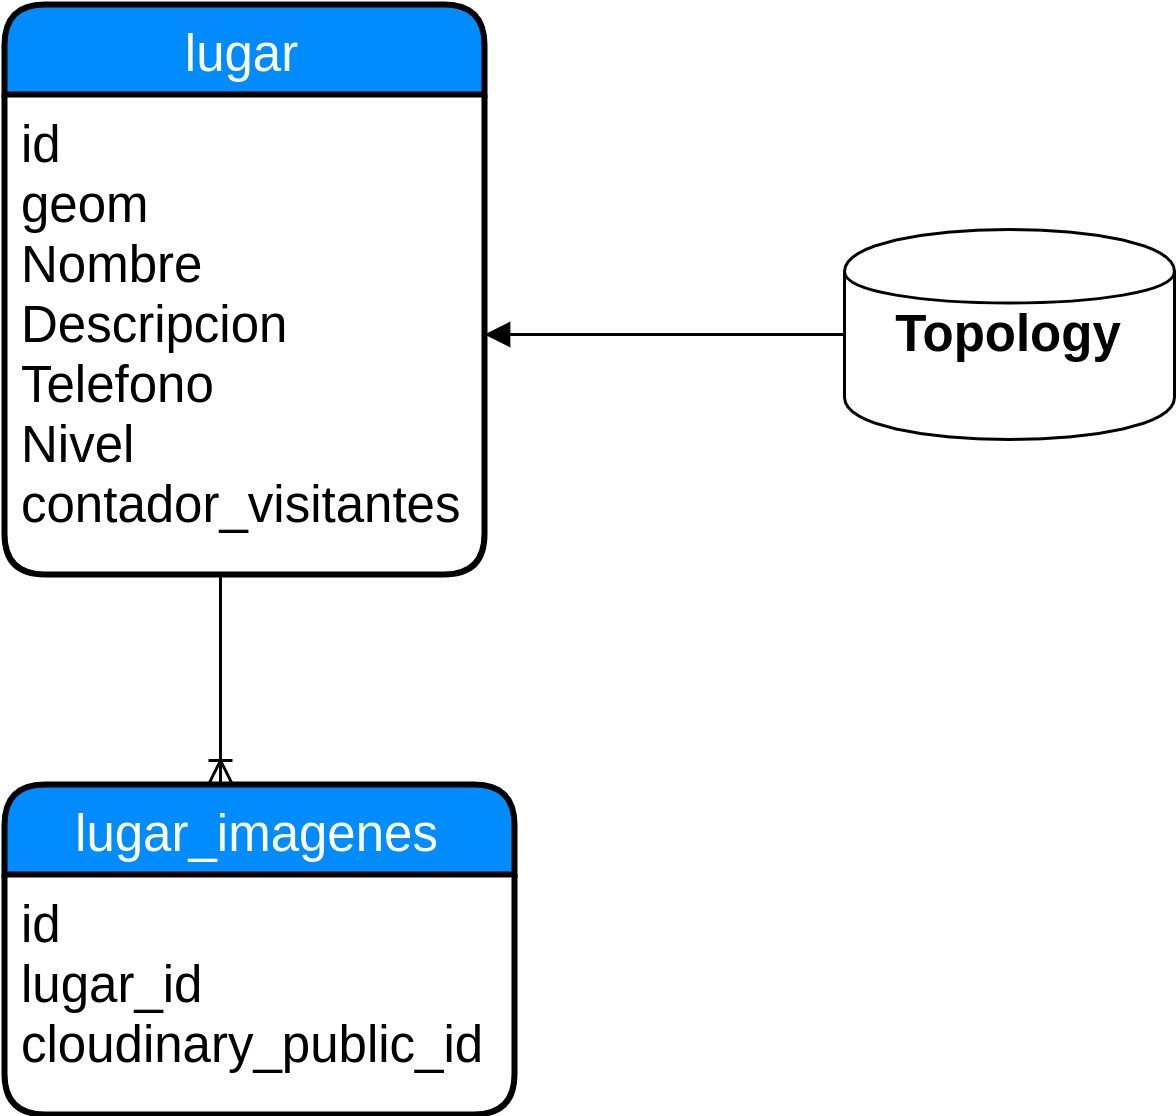
\includegraphics[width=0.4\textwidth]{diagramas/er_lugar}
  \end{center}
  \caption{Diagrama ER: Lugares}
  \label{fig:er_lugar}
  \caption*{Fuente: Elaboración propia}
\end{figure}



\item \textbf{Diagrama de Secuencia:}

En la figura \ref{fig:sequence_ver_lugar}, se observa el diagrama de secuencia correspondiente obtención de la lista e información de lugares.


\begin{figure}[H]
  \begin{center}
    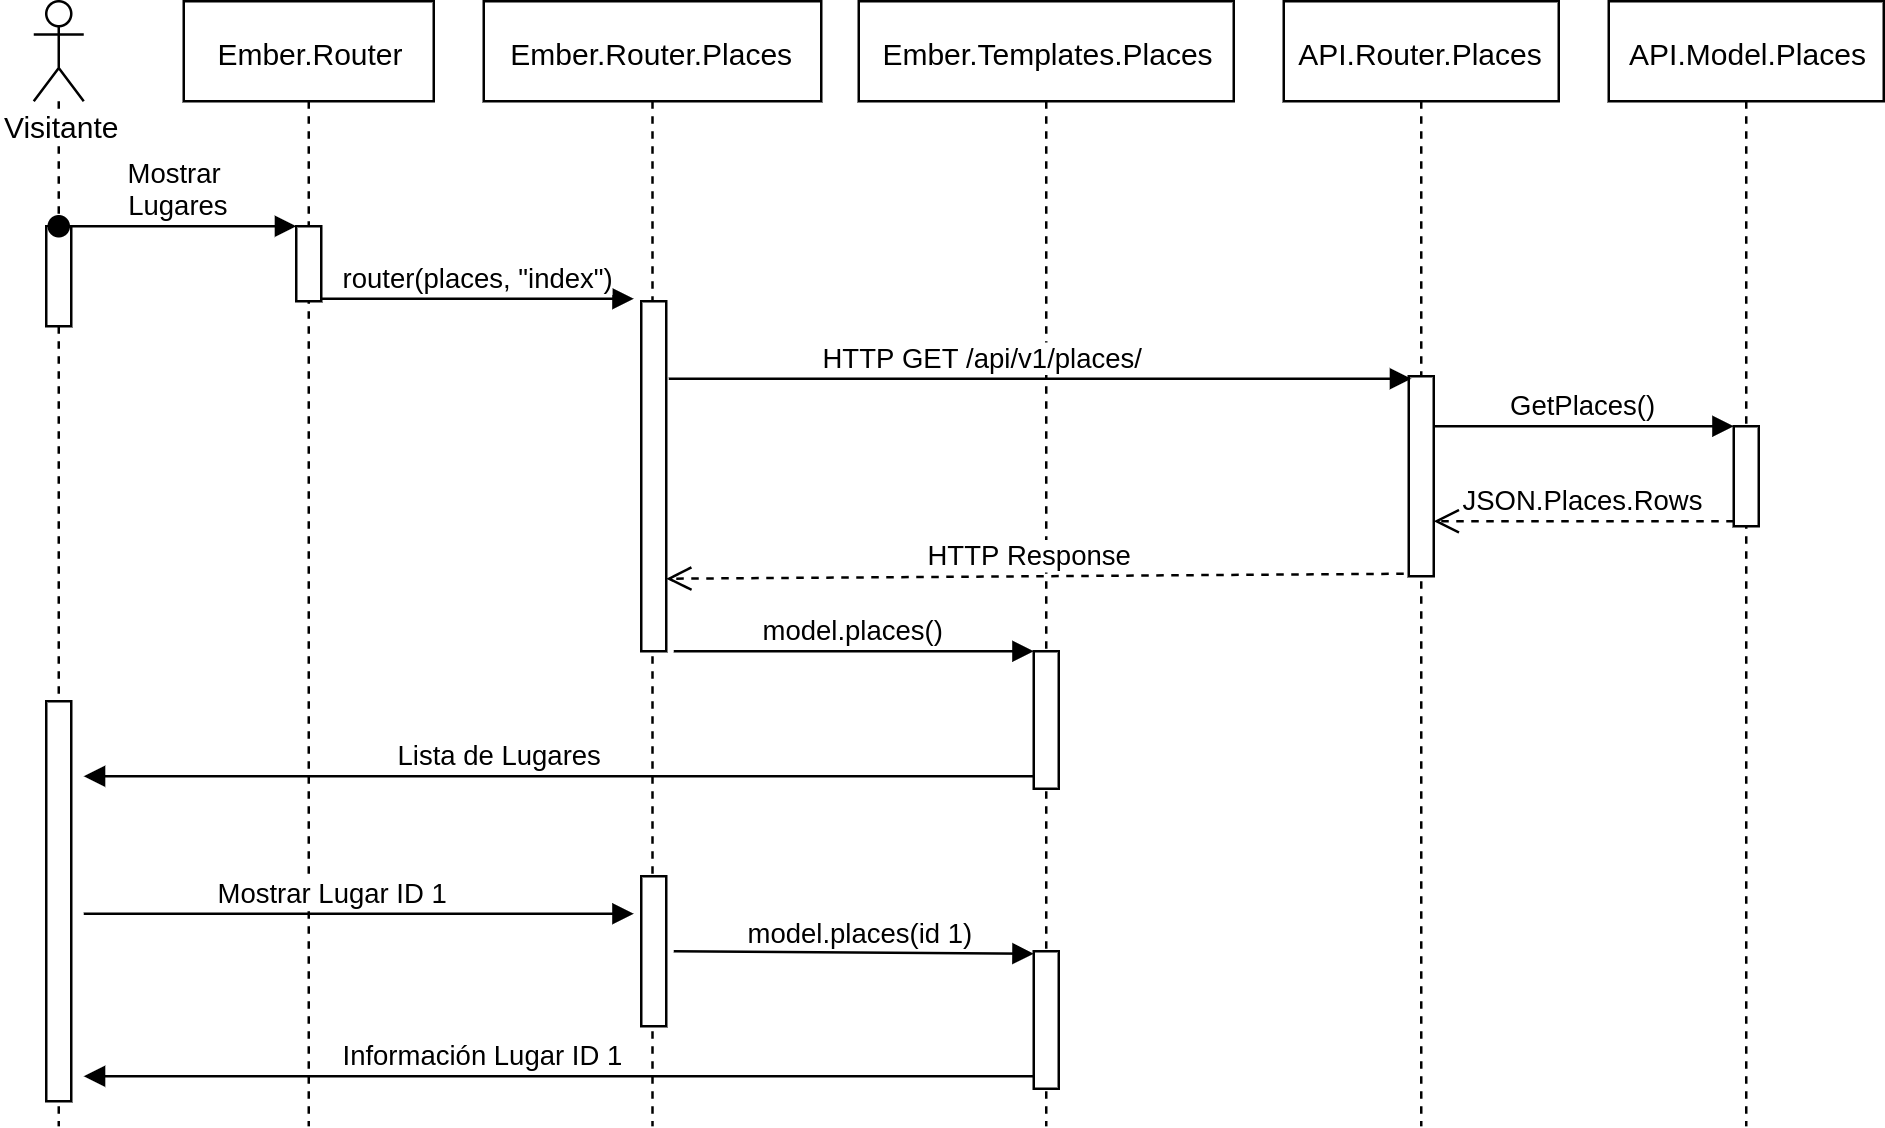
\includegraphics[width=0.9\textwidth]{diagramas/sequence_ver_lugar}
  \end{center}
  \caption{Diagrama de Secuencia: Lista e Información de Lugares}
  \label{fig:sequence_ver_lugar}
  \caption*{Fuente: Elaboración propia}
\end{figure}



\item \textbf{Diagrama de Clases:}


En la figura \ref{fig:clases_lugares}, se observa el diagrama de clases correspondiente a los lugares y la información de estos.

\begin{figure}[H]
\begin{center}
  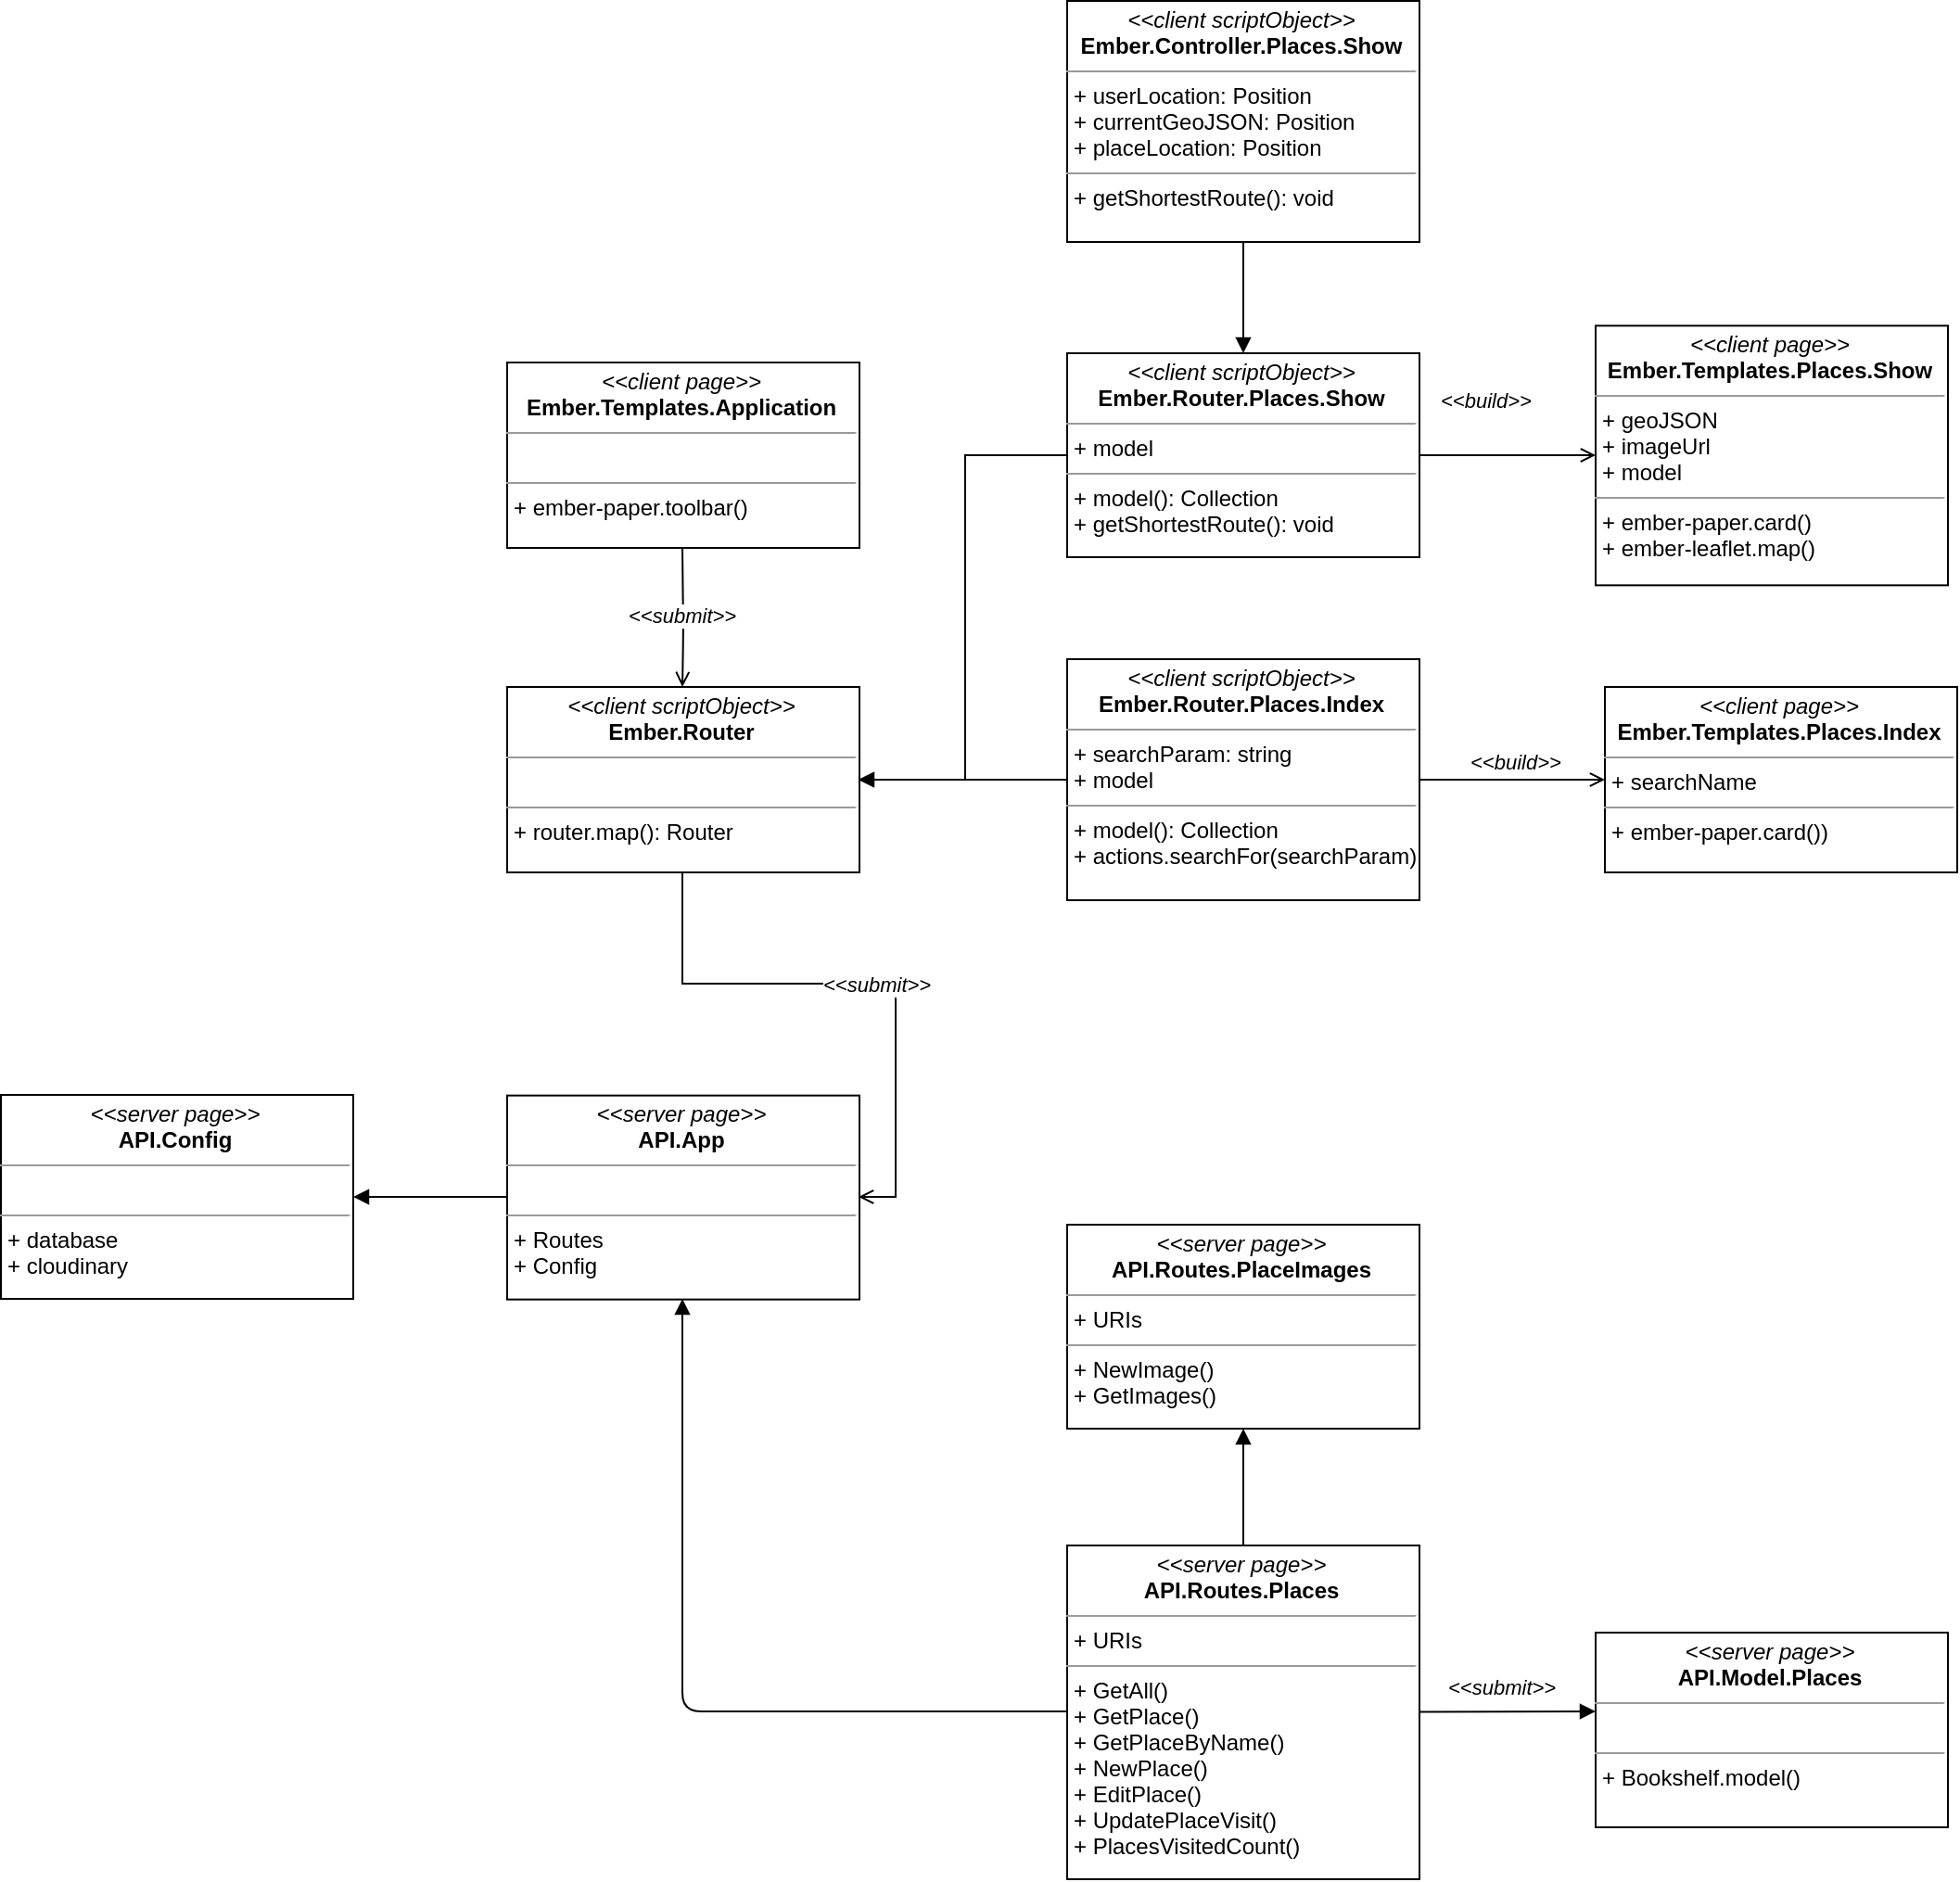
\includegraphics[width=0.9\textwidth]{diagramas/clases_lugares}
\end{center}
\caption{Diagrama de Clases: Lugares}
\label{fig:clases_lugares}
\caption*{Fuente: Elaboración propia}
\end{figure}


\end{itemize}


\subsection{Implementación}
% \label{sub:implementacion_iteracion_1}

    \subsubsection{Recolecion de la informacion de los lugares}
% \label{subs:Los lugares}

En primer lugar se recolectó la información de los lugares que la aplicación contendrá  de forma inicial, al igual que para recolectar las rutas se hizo uso de un \emph{GPS Garmin Nuvi 1300}, el cual cuenta con la opción de guardar locaciones como favoritos, entonces solo fue necesario estar cerca del lugar que se desea guardar y activar esa opción del GPS, este guarda la información en un archivo \emph{.gpx} y con la ayuda de \emph{QGIS} se genero el archivo shapefile correspondiente.\\

Posteriormente es necesario pasar la información geoespacial del shapefile a la base de datos, para esta tarea se hizo uso de una herramienta disponible para postgres, \emph{shp2pgsql}, que permite la conversión de un archivo shapefile a un archivo sql.

% $ shp2pgsql -s 4326 -I -S -c -d ~/Documents/places.shp > places.sql
\begin{verbatim}
  $ shp2pgsql -s 3785 -I -S -c -d ~/Documents/places.shp > places.sql
\end{verbatim}

Con el anterior comando se tiene como resultado un archivo \emph{.sql}, el cual es ingresado en la base de datos ya configurada, de esta forma nuestra base de datos para a contener una tabla geoespacial con datos de tipo \emph{POINT}, los cuales representan los lugares dentro del campus de la UMSS.\\

% \begin{verbatim}
%   $ shp2pgsql -s 4326 -I -S -c -d ~/Documents/ways.shp > ways.sql
% \end{verbatim}
%
% De la misma forma es necesario pasar la información de las rutas contenidas en un archivo shapefile a un archivo sql, en este caso creará una tabla \emph{WAYS}.\\

El archivo \emph{sql} resultante es usado para popular la base de datos con la información inicial de los lugares que contiene el campus universitario, para tal tarea se usó el siguiente comando.\\
% Los archivos resultantes \emph{sql} son usados para popular la base de datos .\\

\begin{verbatim}
  $ psql -d db_ubikate -U db_admin -f /Documents/places.sql
\end{verbatim}

\begin{figure}[H]
  \begin{center}
    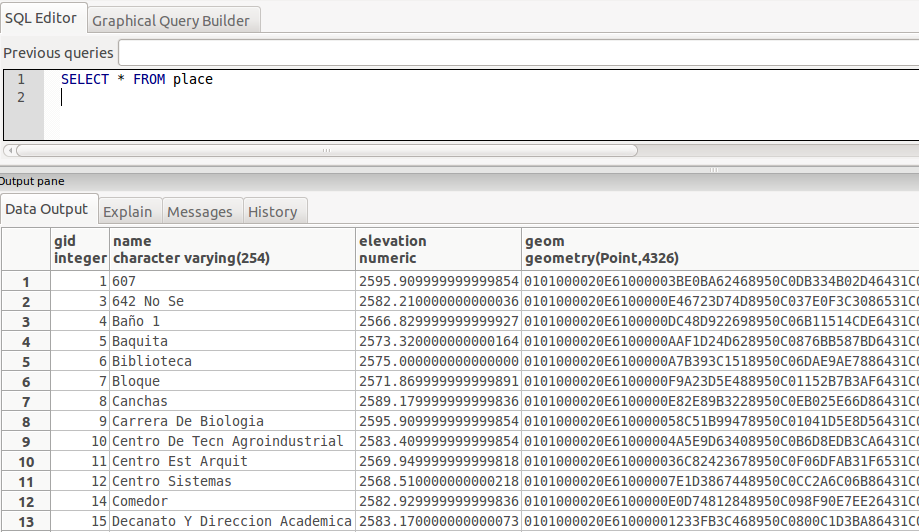
\includegraphics[width=1\textwidth]{iteration1/postgres_places}
    \caption{Herramienta gráfica de PostgreSQL (\emph{pgAdmin}).}
    \label{fig:postgres_places}
    \caption*{Fuente: Elaboración propia}
  \end{center}
\end{figure}
 % con la tabla de Lugares desplegada.

En la figura \ref{fig:postgres_places} se puede observar que la columna \emph{Elevation} contiene datos que el GPS Garmin Nuvi 1300 genera al momento de guardar un punto, en el presente caso es irrelevante.\\


Una vez que se tiene populada la base de datos con la informacion de los lugares es necesario implementar el como se comunicara el backend con el frontend, este como ya se explico se implementara un Servicio Web basado en un API REST.\\



\subsubsection{Implementación del REST API}
\label{subs:Implementacion del REST API}



El servidor necesita reconocer las peticiones que le llegan del cliente, para lo cual es necesario ``mapear'' un URI a una acción específica, las cuales ya están preparadas para comunicarse con la base de datos, no hay restricción en la declaración de las URIs pero para una mejor comprensión del API que se está desarrollando es necesario seguir convenciones que aseguran que cualquier desarrollador pueda comprender el API presentado y pueda ser fácilmente consumido por cualquier aplicación que requiera acceder a la información que disponible, un API REST es el que cumple con estas características.
En primer lugar es necesario crear las URIs que serán ``entendidas'' por el servidor, esto se logra declarando en el servicio creado con \emph{Express.JS}, tal como se puede apreciar en el siguiente bloque de código, cada URI se lo relaciona a un modelo en específico de acuerdo a la acción que se requiere, tal como se puede observar en el cuadro \ref{tab:rest} las URIs declaradas en el API cumplen con tal característica.\\


% \begin{minted}{js}[label=express_api,caption=Declarando API REST con ExpressJS]
\begin{center}
  \begin{lstlisting}[label=express_api,caption=Declarando API REST con ExpressJS]

        const router = express.Router();
        router.get('/', places.getAll);
        router.get('/:id', places.getPlace);
        router.post('/', places.newPlace);
        router.put('/:id', places.editPlace);
        router.delete('/:id', places.deletePlace);

        app.use('/api/v1/places', router);

  \end{lstlisting}
\end{center}
% \end{minted}

% En el código

  %
  % Para lograr todo este comportamiento  es necesario declarar, en el archivo
  % que controla las rutas dentro de la aplicación, \textbf{routes}, que el
  % recurso \textbf{user} es \emph{restful}, tal como se muestra en la figura \ref{fig:rest}\\

  % \begin{figure}[!hbp]
  %   \begin{center}
  %     \caption[REST - routes.rb]{config/routes.rb}
  %     \label{fig:rest}
  %     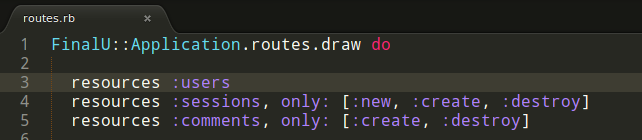
\includegraphics[width=1\textwidth]{rest}
  %     \caption*{Fuente: }
  %   \end{center}
  % \end{figure}

  El cuadro \ref{tab:rest} muestra como se puede leer las peticiones al API de \textbf{places}, las acciones mostradas son las que se pueden encontrar en un API REST pero no es necesario declararlas todas para considerar a que un API es restful.\\


  \begin{table}[H]
    \begin{center}

      \begin{tabularx}{0.75\textwidth}{ l l l  X }
        \toprule
        \multicolumn{1}{c}{\textbf{HTTP}} &
        \multicolumn{1}{c}{\textbf{URI}}  &
        % \multicolumn{1}{c}{\textbf{C}}  &
        \multicolumn{1}{c}{\textbf{ACCI\'ON}} &
        \multicolumn{1}{c}{\textbf{USADO PARA}}  \\
        \multicolumn{1}{c}{\textbf{request}} & & & \\

        \midrule
        GET     &  /places    &  index    & devuelve una lista con todos los lugares\\
        POST    &  /places    &  create   & inserta un nuevo lugar en la bd\\
        GET     &  /places/1  &  show     & muestra el lugar con identificador \emph{1}\\
        PUT     &  /places/1  &  update   & actualiza los datos de un lugar específico\\
        DELETE  &  /places/1  &  delete   & elimina el lugar con id = 1 de la bd\\
        \bottomrule
      \end{tabularx}

      \caption[recursos REST]{REST URIs para los lugares}
      \label{tab:rest}

      \caption*{Fuente: Elaboración propia}
    \end{center}
  \end{table}

  % Tal como se ve en el cuadro \ref{tab:rest}, Rails maneja los request HTTP de acuerdo con
  % el tipo de llamada que se realice, este trabajo lo realiza el \textbf{router},
  % que reconoce las URLs y los despacha a una \textbf{acción} del controlador,
  % todo este proceso ya está implementado en el núcleo de Rails por lo tanto  es automático y el programador
  % no necesita más configuración que la mostrada en la figura \ref{fig:rest},
  % obedeciendo al principio de \emph{Convención sobre configuración}\\

  % % no son más que métodos dentro del \emph{user\_controller.rb}
  % el cual
  % es parte del controlador de la arquitectura MVC.\\

  % The Rails router recognizes URLs and dispatches them to a controller’s action. It can also generate paths and URLs, avoiding the need to hardcode strings in your views.

  Por ejemplo, si se genera una petición GET hacia la direccion
  \mbox{\emph{/places/1}}  el servidor interpreta la dirección y responde
  mostrando la información del lugar “1” y en cambio si se genera
  una petición \emph{PUT} a la misma direccion \emph{/places/1} se ejecuta la acción \textbf{update} y se actualizan los datos del lugar ``1''. \\

  % \textbf{usuarios} actualizando la información del usuario “1”. \\

  Siguiendo la convención de un API REST ayuda a entender el flujo que tiene un recurso,
  las URL son legibles y únicos para cada recurso. Por lo tanto la implementación   de los recursos se hace de forma más limpia y ordenada, situaciones que son   claves para el mantenimiento y la extensibilidad del sistema. \\


Una vez implementado el servicio web, necesitamos empezar con el desarrollo del frontend de la aplicacion, que como ya se explico se usara \emph{EmberJS} para esta tarea. \\


\subsubsection{Mostrar los lugares}


\emph{EmberJS} tiene que consumir la informacion del API implementado, por lo tanto se hara una llamada \emph{GET} al URI \emph{places/}, dentro de la estructura de \emph{EmberJS} se tiene que implementar en el \emph{Router} dedicado al URI correspondiente. El siguiente metodo es el encarado de hacer la llamada y obtener la lista de lugares del API

\begin{center}
  \begin{lstlisting}[label=model_places_index,caption=Obtener la lista de lugares del API]

    model() {
        var url = (ENV.APP.API_HOST || '') + '/api/v1/places/';
        return jQuery.ajax({
          url: url,
          type: 'GET'
        });
      }

  \end{lstlisting}
\end{center}

Una vez obtenido la lista de lugares es necesario para el visitante que la lista este disponible en el navegador, para lo cual se usara el \emph{template} de \emph{EmberJs} correspondiente al URI, \emph{templates/places/index.hbs}.

\begin{center}
  \begin{lstlisting}[label=template_places_index,caption=Template de la lista de lugares]

    {{#paper-list}}
      {{#each model.data as |place|}}
        {{#paper-item class="md-1-line" onClick=(transition-to 'places.show' place)}}
            <div class="md-list-item-text">
                <span>{{place.name}}</span>
            </div>
        {{/paper-item}}
        {{paper-divider}}
      {{/each}}
    {{/paper-list}}

  \end{lstlisting}
\end{center}

En la anterior implementacion se hizo uso de \emph{ember-paper}, que como ya se explico ayudara en el ``look and feel'' de la aplicacion, el cual se puede observar en la figura \ref{fig:places_index}, la lista de lugares es mostrada en el navegador en un dispositivo movil.


\begin{figure}[H]
  \begin{center}
    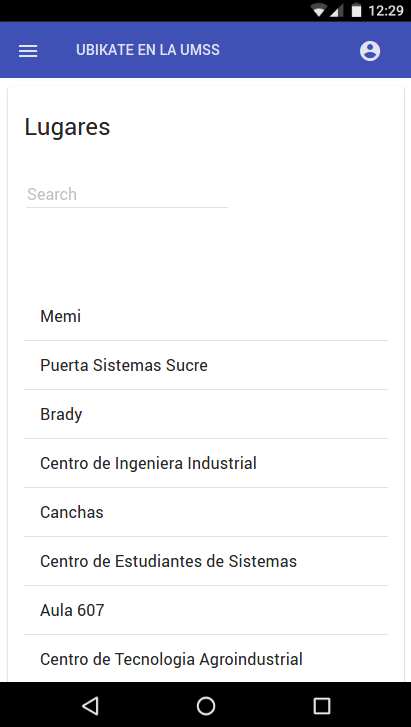
\includegraphics[width=0.3\textwidth]{iteration1/places_index_2}
    \caption{Lista de Lugares}
    \label{fig:places_index}
    \caption*{Fuente: Elaboración propia}
  \end{center}
\end{figure}


\subsubsection{Busqueda de los lugares}
\label{subs:busqueda de los lugares}

Para la implementacion de la busqueda de los lugares, un de los criterios de aceptacion es que sea posible la busqueda usando el nombre del lugar o parte del mismo, es necesario anadir un \emph{URI} adicional a nuestro servicio web, que obtenga de la base de datos un conjunto de lugares que concuerden con el criterio de busqueda, a continuacion se puede ver el URI implementado en la servicio web. \\

\begin{center}
  \begin{lstlisting}[label=endpoint_search_place,caption=Implementacion de la busqueda de lugares en el Servicio Web]

    router.get('places/search/:name', places.getPlacesByName);

  \end{lstlisting}
\end{center}


\subsubsection{Mostrar informacion del lugar}
\label{subs:Mostrar informacion del lugar}

La obtencion de la informacion de un lugar corresponde al URI \emph{places/:id} usando el verbo HTTP \emph{GET}, el cual obtiene la informacion en formato JSON, entonces se necesita mostrar esta informacion en el navegador, para lo cual el template correspondente al URI llegaria a ser \emph{templates/places/show}.

\begin{center}
  \begin{lstlisting}[label=template_places_show,caption=Template para mostrar la informacion de un lugar]
      {{#text.headline}}{{model.name}}{{/text.headline}}
      {{#card.content}}
          {{#paper-list}}
              {{model.description}}
              {{/paper-item}}
                  {{paper-icon "local_phone"}} {{model.phone}}
              {{/paper-item}}
              {{#paper-item class="md-2-line" }}
                  {{paper-icon "layers"}} Piso N# {{model.level}}
              {{/paper-item}}
          {{/paper-list}}
      {{/card.content}}

  \end{lstlisting}
\end{center}

El resultado del template renderizado en el navegador se puede apreciar en la figura \ref{fig:place_show}.

\begin{figure}[H]
  \begin{center}
    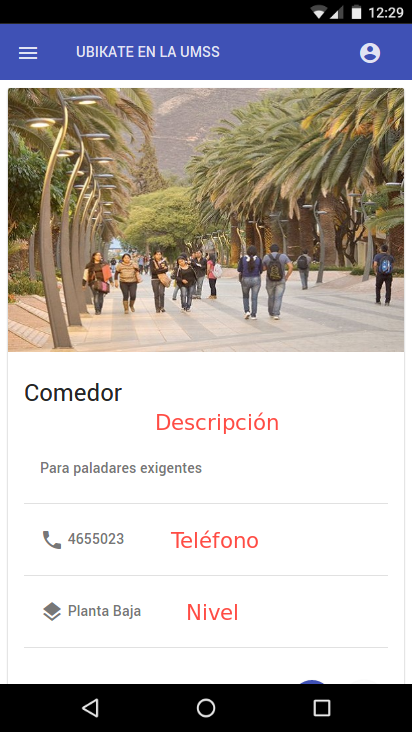
\includegraphics[width=0.3\textwidth]{iteration1/place_show}
    \caption{Vista de la Información de un Lugar.}
    \label{fig:place_show}
    \caption*{Fuente: Elaboración propia}
  \end{center}
\end{figure}




% En la figura \ref{fig:places_index}, se puede observar un


\subsection{Pruebas de Aceptación}

\begin{table}[H]
  \begin{center}
    \begin{tabularx}{0.75\textwidth}{ X }
      \toprule
      \textbf{Codigo:} CP001
      \makebox[3cm][r]{}
      \makebox[6cm][r]{\textbf{Historia de Usuario:} US01} \\

      \addlinespace
      \textbf{Nombre:} Verificar la lista de lugares. \\

      \addlinespace
      \textbf{Descripción:} Validar que un usuario visitante puede ver la lista de lugares cuando ingresa al menú \emph{lugares}. \\

      \addlinespace
      \textbf{Condiciones de Ejecución:} \\
      \tab \textbf{a.} El usuario no debe estar registrado. \\
      \tab \textbf{b.} Deben existir lugares registrados en el sistema.\\

      \addlinespace
      \textbf{Entradas / Pasos de Ejecución:}  \\
      \tab \textbf{1.} Hacer tap sobre el botón \emph{menú} en la esquina superior-izquierda. \\
      \tab \textbf{2.} Seleccionar el menú \emph{lugares}.\\

      \addlinespace
      \textbf{Resultado Esperado:} El Usuario debe ver una lista con los lugares registrados en la Condición de Ejecución \emph{b}.  \\

      \addlinespace
      \textbf{Evaluación de la Prueba:} Prueba exitosa. \\

      \bottomrule
    \end{tabularx}
    \caption{Prueba de Aceptación - CP001}
    \label{tab:CP001}
  \end{center}
\end{table}

\begin{table}[H]
  \begin{center}
    \begin{tabularx}{0.75\textwidth}{ X }
      \toprule
      \textbf{Codigo:} CP002
      \makebox[3cm][r]{}
      \makebox[6cm][r]{\textbf{Historia de Usuario:} US01} \\

      \addlinespace
      \textbf{Nombre:} Verificar la busqueda de lugares. \\

      \addlinespace
      \textbf{Descripción:} Validar que un usuario puede filtrar un lugar de la lista mediante el nombre. \\

      \addlinespace
      \textbf{Condiciones de Ejecución:} Ingresar en la base de datos el lugar con nombre ``MEMI''. \\

      \addlinespace
      \textbf{Entradas / Pasos de Ejecución:}  \\
      \tab \textbf{1.} Hacer tap sobre el botón \emph{menú} en la esquina superior-izquierda. \\
      \tab \textbf{2.} Seleccionar el menú \emph{lugares}.\\
      \tab \textbf{3.} Ingresar el nombre ``MEMI'' en el cajón de búsqueda.\\


      \addlinespace
      \textbf{Resultado Esperado:} Se debe mostrar un solo item en la lista de lugares con el nombre ``MEMI'' desplegado.\\

      \addlinespace
      \textbf{Evaluación de la Prueba:} Prueba exitosa. \\

      \bottomrule
    \end{tabularx}
    \caption{Prueba de Aceptación - CP002}
    \label{tab:CP002}
  \end{center}
\end{table}

\begin{table}[H]
  \begin{center}
    \begin{tabularx}{0.75\textwidth}{ X }
      \toprule
      \textbf{Codigo:} CP003
      \makebox[3cm][r]{}
      \makebox[6cm][r]{\textbf{Historia de Usuario:} US02} \\

      \addlinespace
      \textbf{Nombre:} Verificar la información de un lugar. \\

      \addlinespace
      \textbf{Descripción:} Validar que un usuario puede ver la descripción, el teléfono, el nivel y la foto de un lugar. \\

      \addlinespace
      \textbf{Condiciones de Ejecución:} Ingresar en la base de datos el lugar con nombre ``MEMI'' con su información completa. \\

      \addlinespace
      \textbf{Entradas / Pasos de Ejecución:}  \\
      \tab \textbf{1.} Hacer tap sobre el botón \emph{menú} en la esquina superior-izquierda. \\
      \tab \textbf{2.} Seleccionar el menú \emph{lugares}.\\
      \tab \textbf{3.} En la lista de lugares seleccionar el item ``MEMI''.\\

      \addlinespace
      \textbf{Resultado Esperado:} Se debe mostrar una pantalla con la foto del lugar ``MEMI'', su descripción, el teléfono y el nivel.\\

      \addlinespace
      \textbf{Evaluación de la Prueba:} Prueba exitosa. \\

      \bottomrule
    \end{tabularx}
    \caption{Prueba de Aceptación - CP003}
    \label{tab:CP003}
  \end{center}
\end{table}



\subsubsection{Resultado de las pruebas de la Iteración 1}

Al finalizar la Iteración 1, se ejecutaron todas las pruebas escritas durante la presente iteración, en el cuadro \ref{tab:regresion_1} se puede ver el detalle.


\begin{table}[H]
  \begin{center}
    \begin{tabularx}{0.8\textwidth}{ c  X  c }
      \toprule
        \textbf{Código} &
        \multicolumn{1}{c}{\textbf{Título de la Prueba}} &
        \textbf{Resultado}\\

      \midrule
        CP001
        &
        Verificar la lista de lugares.
        &
        Exitoso \\

\addlinespace
CP002
&
Verificar la busqueda de lugares.
&
Exitoso \\

\addlinespace
CP003
&
Verificar la información de un lugar.
&
Exitoso \\

\addlinespace
CP004
&
Verificar la lista de lugares cuando se busca un lugar no registrado.
&
Exitoso \\

\addlinespace
CP005
&
Verificar la información de un lugar mediante el URI.
&
Exitoso \\

\addlinespace
CP006
&
Verificar que el \emph{Menú} sea desplegado dinámicamente.
&
Exitoso \\



      \bottomrule
    \end{tabularx}
    \caption{Pruebas de regresión de la Iteración 1}
    \label{tab:regresion_1}
  \end{center}
\end{table}


\begin{itemize}
  \item Se ejecutaron 5 pruebas de funcionalidad, todas pasaron exitosamente.
  \item Se ejecutó 1 prueba de usabilidad, pasó exitosamente.
\end{itemize}



\section{Iteración 2}
\label{sec:iteracion_2}

Después de que finalizó la primera iteración y ya que todas las pruebas pasaron exitosamente, se continúa con la segunda iteración.


\subsection{Iteration Planning Meeting}
\label{sub:iteration2_planning_meeting}


Al igual que la primera iteración, las fases de exploración y planeación se realizan al mismo tiempo, en el sentido que no es necesario repartir las tareas resultantes de la exploración, por lo tanto al mismo tiempo en que se determinan las tareas se puede realizar la estimación de las mismas.

  \subsubsection{Exploración y Planeación}
  \label{subs:iteration2_exploracion_planeacion}

  Para la segunda iteración se toman en cuenta todas las historias de usuario restantes, y de acuerdo al criterio de escoger las siguientes historias más relevantes y de mayor valor para el producto, se escogió la historia de usuario #4.\\

  Como parte de la fase de Exploración se toma la historia de usuario #4 y la dividimos en las Tareas de Ingeniería, las cuales serán trabajadas en la fase de la Implementación.

  En la siguente tabla se especificaran las tareas correspondientes a la historia de usuario #4 \ref{tab:us04_tasks}. \\

  \subsection{Tareas del US04}
  \label{sub:us04_tasks}

    \begin{table}[H]
  \begin{center}
    \begin{tabularx}{\textwidth}{ c  X  C{2.3cm} }
      \toprule
        \textbf{Código} &
        \multicolumn{1}{c}{\textbf{Tarea}} &
        \textbf{Estimación [dias]}\\

      \midrule
        T011
        &
        Crear un archivo shapefile con información inicial de lugares principales dentro el campus de la UMSS.
        &
        2 \\

      \addlinespace
        T012
        &
        Preparar la base de datos para manejar información geográfica de rutas.
        &
        1 \\
      %
      % \addlinespace
      %   T013
      %   &
      %   Investigar e instalar una herramienta que permita usar un servicio de mapas.
      %   &
      %   1 \\

      % \addlinespace
      %   T014
      %   &
      %   El usuario puede ver un mapa usando un servicio del campus de la UMSS.
      %   &
      %   0.5 \\

      % \addlinespace
      %   T015
      %   &
      %   El usuario puede ver un marcador sobre el lugar.
      %   &
      %   0.5 \\
      %
      % \addlinespace
      %   T016
      %   &
      %   El marcador tiene información básica del lugar, nombre, piso.
      %   &
      %   0.5 \\

      \addlinespace
        T017
        &
        El usuario puede ver un marcador mostrando el lugar actual donde se encuentra (el usuario).
        &
        0.5 \\

      \addlinespace
        T018
        &
        Desarrollar un módulo que encuentra la ruta más corta usando la base de datos con información geográfica ruteable de T012.
        &
        2 \\

      \addlinespace
        T019
        &
        El usuario puede ver una línea roja que une el marcador de la posición del usuario con el marcador del lugar.
        &
        1 \\

      % \addlinespace
      %   TS003
      %   &
      %   Crear pruebas de funcionalidad del US04.
      %   &
      %   1 \\

      \addlinespace
      \midrule
        & \multicolumn{1}{R{7cm}}{\textbf{Total: }}
        & 10 \\

      \bottomrule
    \end{tabularx}
    \caption{Tareas del US04}
    \label{tab:us04_tasks}
  \end{center}
\end{table}


  \subsection{Calendario de Entregas}
  \label{subs:schedule_2}

    % \begin{table}[!ht]
%
% \end{table}
\begin{table}[H]

  \begin{center}

\begin{ganttchart}[
  canvas/.append style={fill=none, draw=black!5, line width=.75pt},
  hgrid style/.style={draw=black!5, line width=.75pt},
  vgrid={*1{draw=black!5, line width=.75pt}},
  %today=0,
  % today label=Semana 3,
  today rule/.style={
    draw=black!64,
    dash pattern=on 3.5pt off 4.5pt,
    line width=1.5pt
  },
  today label font=\small\bfseries,
  title/.style={draw=none, fill=none},
  title label font=\bfseries\footnotesize,
  title label node/.append style={below=7pt},
  include title in canvas=false,
  bar label font=\mdseries\small\color{black!70},
  bar label node/.append style={left=2cm},
  bar/.append style={draw=none, fill=black!63},
  bar incomplete/.append style={fill=barblue},
  bar progress label font=\mdseries\footnotesize\color{black!70},
  group incomplete/.append style={fill=groupblue},
    group left shift=0,
    group right shift=0,
    group height=.5,
    group peaks tip position=0,
    group label node/.append style={left=.6cm},
    group progress label font=\bfseries\small,
    link/.style={-latex, line width=1.5pt, linkred},
    link label font=\scriptsize\bfseries,
    link label node/.append style={below left=-2pt and 0pt},
  ]{1}{12}
  \gantttitle{Calendario de Entregasde de la Iteración 2}{7} \\[grid]
  \gantttitle{Semana 1}{7}
  \gantttitle{Semana 2}{7} \\
  % \gantttitle{Noviembre}{4} \\
  \gantttitle[title label node/.append style={below left=7pt and -3pt}]{D\'ia:\quad15}{0}
  \gantttitlelist{16,...,30}{1} \\
  % \ganttgroup[progress=0]{Historias de Usuario}{1}{8} \\
  \ganttbar[
    progress=0,
    name=bar1
  ]{\textbf{User Story 04}}{1}{12} \\
  % \ganttbar[
  %   progress=0,
  %   name=bar2
  % ]{\textbf{User Story 03}}{10}{12} \\
  % \ganttbar[
  %   progress=0,
  %   name=bar3
  % ]{\textbf{Iteración 3}}{5}{6} \\
  % \ganttbar[
  %   progress=0,
  %   name=bar4
  % ]{\textbf{Iteración 4}}{7}{8} \\
  % \ganttbar[
  %   progress=100,
  %   name=bar5
  % ]{\textbf{Actividad 5}}{5}{7} \\
  % \ganttbar[
  %   progress=80,
  % ]{\textbf{Actividad 6}}{8}{8} \\
  % \ganttbar[
  %   progress=49,
  % ]{\textbf{Actividad 7}}{9}{11} \\
  % \ganttmilestone{Hito 1}{11}{11}  \\
  % \ganttmilestone{Hito 2}{12}{12} \\
  %

  % \ganttmilestone{Q6 report}{24}{24} \\
  % \ganttmilestone{M1: Project finished}{8}{8}

  % \ganttlink[link type=f-s]{bar1}{bar2}
  % \ganttlink[link type=f-s]{bar2}{bar3}
  % \ganttlink[link type=f-s]{bar3}{bar4}

\end{ganttchart}

\caption{Calendario de Entregas de la Iteración 2}
\label{tab:calendario_entregas_iteracion_2}

\end{center}
\end{table}



\subsection{Implementación}
\label{sub:implementacion_iteracion_1}

Durante esta fase es donde se implementaran las tareas especificadas en la tabla \ref{tab:us04_tasks}.

\subsubsection{RF011}
\label{subs:RF011}

% Crear un archivo shapefile con la información geográfica de las rutas internas del campus de la UMSS

% Como ya se explico en \ref{sec:ruta_corta_umss}, esta tarea se llevo a cabo recabando la informacion geoespacial con un dispositivo GPS y exportando los datos resultantes a un archivo shapefile, el cual se puede apreciar en \ref{fig:shapefile_umss_v1}.

\subsubsection{RF012}
\label{subs:RF012}

% Preparar la base de datos para manejar información geográfica de rutas

% Para realizar esta tarea se procedió a instalar pgRouting, el resultado de esta tarea se puede apreciar en el manual de instalación ## \\
%
% Una vez configurada la base de datos se procede a cargar la misma con la informacion obtenida en RF011, para tal efecto es necesario primeramente crear una tabla que contendra los LINESTRING contenidos en el shapefile, esta operacion es similar a la realizada en la tarea - RF003 (\ref{sub:RF003}). Una vez que ya se tiene la tabla a la llamamos \emph{ways}, se necesita ejecutar un query propio de \emph{pgRouting} el cual tiene como objetivo analizar los datos geo-espaciales de la tabla y a\~nadirle una \emph{topologia}.
%
% Dentro lo que es la \emph{topologia geoespacial} existe una aplicacion que se lo conoce como \emph{topología de red}. La \emph{topología de red} representa las relaciones entre segmentos en una red lineal o una colección de segmentos de línea\cite{osgeo_journal_topology}.
% En un \emph{SIG} la topologia ayuda a mejorar el analisis de datos geo-espaciales, para resolver el problema de la ruta corta \emph{pgRouting} genera una \emph{topología de red} usando los datos que existen en la tabla \emph{ways}, es necesario ejecutar una instruccion, la que se muestra a continiacion y \emph{pgRouting} se encarga de llenar los datos que se pueden observar en la figura \ref{fig:postgres_ways}, las columnas \emph{source} y \emph{target} son populadas con el analisis topologico y en la figura \ref{fig:postgres_vertices}, se puede observar que la tabla \emph{ways\_vertices\_pgr} es creada enteramente en la ejecucion de la instruccion.
%
% \begin{verbatim}
%   select pgr_createTopology('ways', 0.00000001, 'geom', 'gid');
% \end{verbatim}
%
% \begin{figure}[H]
%   \begin{center}
%     \caption{Vista de la tabla \emph{ways} en la base de datos PostgreSQL.}
%     \label{fig:postgres_ways}
%     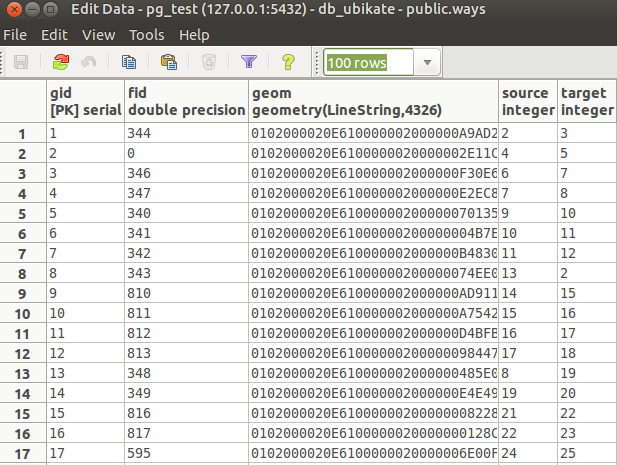
\includegraphics[width=1\textwidth]{iteration2/postgres_ways}
%     \caption*{Fuente: Elaboración propia}
%   \end{center}
% \end{figure}
%
% En la figura \ref{fig:postgres_ways} se puede apreciar que cada fila es una parte de la línea original obtenida por el dispositivo GPS y explisionada por QGIS, hay que notar que las columnas \emph{source} y \emph{target} hacen referencia a los nodos o vertices que la primera linea tiene en sus extremos, la primera linea o fila esta identificada por la columna \emph{gid}.\\
%
% En la siguiente figura \ref{fig:postgres_vertices} se observa la tabla \emph{ways\_vertices\_pgr} que contiene los vertices creados a partir del analisis de los datos en la tabla \emph{ways}.
%
% \begin{figure}[H]
%   \begin{center}
%     \caption{Vista de la tabla \emph{ways\_vertices\_pgr} en la base de datos PostgreSQL.}
%     \label{fig:postgres_vertices}
%     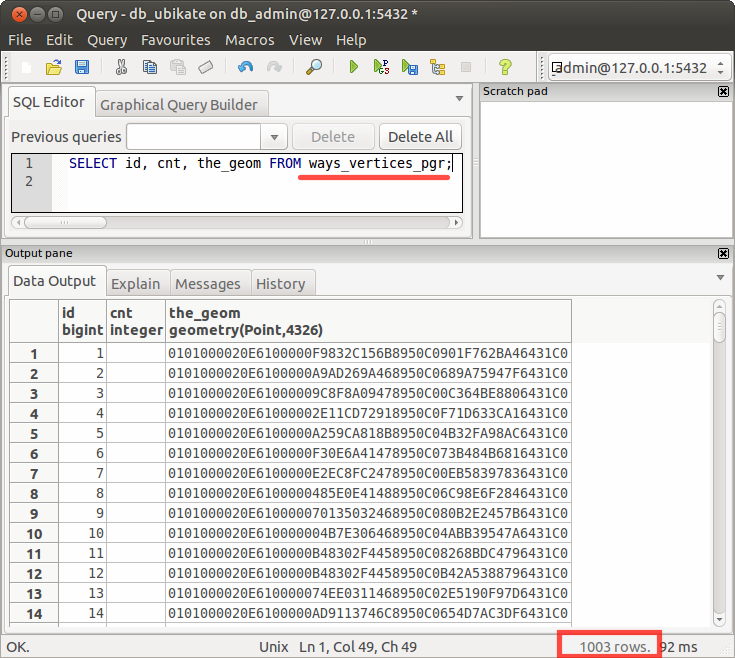
\includegraphics[width=1\textwidth]{iteration2/postgres_vertices}
%     \caption*{Fuente: Elaboración propia}
%   \end{center}
% \end{figure}
%
% Para entender los datos generados hay leer la informacion de las 2 tablas, por ejemplo en la primera  fila (gid 1) de la tabla \emph{ways}, se observa que el contenido de la columna \emph{source} es igual a \textbf{2} y \emph{target} es igual a \textbf{3}, eso quiere decir que los vertices del LINESTRING de la fila 1 son los vertices con \textbf{id} 2 y 3 respectivamente de la tabla \emph{ways\_vertices\_pgr}.\\
%
%
% Todo el conjunto de vertices y lineas de estas tablas se podria representar con una Matriz de adyacencias, explicada en \ref{sub:representacion_de_un_grafo}, y usada en la resolucion de la ruta mas corta, mas especificamente con el algoritmo de Dijkstra.

\subsubsection{RF013}
\label{subs:RF013}

% Investigar e instalar una herramienta que permita usar un servicio de mapas
% Durante la investigacion de esta tarea se encontro \emph{ember-leaflet}, una libreria o plugin que contiene las herramientas para poder cargar y usar un servicio de mapas.\\
%
% Para instalar esta libreria solo se necesita ejecutar el siguiente comando y posteriormente ya se puede empezar a utilizarla.\\
%
% \begin{verbatim}
%   $ ember install ember-leaflet
% \end{verbatim}
%
% El resultado de la investigacion puede apreciar en el marco teórico, en la sección que describe la librería, \emph{ember-leaflet}. \ref{sec:ember_js}

\subsubsection{RF014}
\label{subs:RF014}

% El usuario puede ver un mapa usando un servicio del campus de la UMSS

% Para completar esta tarea se hizo uso de la herramienta \emph{ember-leaflet}, con la cual se puede desplegar un mapa en el browser y optimizada para dispositivos moviles.\\
%
% \begin{verbatim}
%   {{#leaflet-map lat=lat lng=lng zoom=zoom}}
%     {{tile-layer
%       url="http://{s}.tile.openstreetmap.fr/hot/{z}/{x}/{y}.png"
%     }}
%   {{/leaflet-map}}
% \end{verbatim}
%
% Con la anterior instrucción se accede al servicio de \emph{Open Street Maps}, de la cual obtenemos los datos necesarios para renderizar un mapa en el browser. Los atributos de \emph{lat} y \emph{lng} se acceden de la capa del controlador de la aplicacion, son la latitud y longitud respectivamente, la convinacion de ambos datos es la locacion donde se va a ubicar el renderizado del mapa.\\

% Esta librería es la nos ayudará a insertar fácilmente los marcadores que irán sobre los lugares o la líneas que mostraran la ruta más corta
%
% Como resultado de esta tarea se puede apreciar la siguiente figura,

\subsubsection{RF015}
\label{subs:RF015}
% El usuario puede ver un marcador sobre el lugar

% Para completar esta tarea se continuó usando la librería \emph{ember-leaflet}, la cual permite que con la siguiente instrucción se despliegue un marcador sobre el mapa renderizado del API de \emph{Open Street Maps}.
%
% \begin{verbatim}
%   {{#marker-layer location=userLocation}} {{/marker-layer}}
% \end{verbatim}
%
% El resultado de la tarea se puede observar en la figura \ref{fig:baquita_place}.

\subsubsection{RF016}
\label{subs:RF016}
% marcador se  tiene información básica del lugar, nombre, piso

% Para poder mostrar la informacion del lugar sobre el marcador creado en RF015 se hizo uso de la librería \emph{ember-leaflet}, al igual que dicha tarea, solo se necesito de una instruccion para poder desplegar la informacion necesaria.
%
% \begin{verbatim}
%   {{#marker-layer location=location}}
%     h3>{{model.name}}</h3>
%     {{model.description}}
%     <strong>telf:</strong> {{model.phone}}
%     <strong>piso#</strong> {{model.level}}
%   {{/marker-layer}}
% \end{verbatim}
%
% En la figura \ref{fig:baquita_place} se puede apreciar el marcador con la información desplegada del lugar ``Baquita''.
%
% \begin{figure}[H]
%   \begin{center}
%     \caption{Tooltip con la información de un lugar.}
%     \label{fig:baquita_place}
%     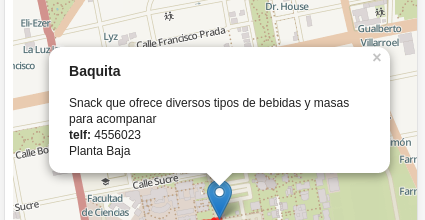
\includegraphics[width=1\textwidth]{iteration2/baquita_place}
%     \caption*{Fuente: Elaboración propia.}
%   \end{center}
% \end{figure}


\subsubsection{RF017}
\label{subs:RF017}
% El usuario puede ver un marcador mostrando el lugar actual donde se encuentra (el usuario)

% Para encontrar la locación del usuario se uso el API de geolocalización propio de HTML5, que en un smarthphone puede acceder y usar los recursos nativos de un smartphone, es necesaria la aceptacion del usuario mediante un mensaje que el navegador desplega, la locacion es encontrada mediante la triangulacion de Coordenadas por GPS (el mas exacto a la hora de encontrar la locacion del dispositvo), Wi-Fi, GSM o CDMA. Solo es necesaria la ejecucion de la siguente linea para ponder obetener la posición actual del usuario usando el API de geolocalización de HTML5.
%
% \begin{verbatim}
%   var coords = Geolocation.getCurrentPosition();
%   var latitud = coords.latitude;
%   var longitud = coords.longitude;
% \end{verbatim}
%
% La \emph{latitud} y \emph{longitud} obtenidas es fácilmente trasladado al mapa usando \emph{ember-leaflet} mediante un marcador, como se puede apreciar en la siguiente figura.
%
% \begin{figure}[H]
%   \begin{center}
%     \caption{Tooltip con la latitud y longitud de la posición actual del usuario.}
%     \label{fig:location_marker}
%     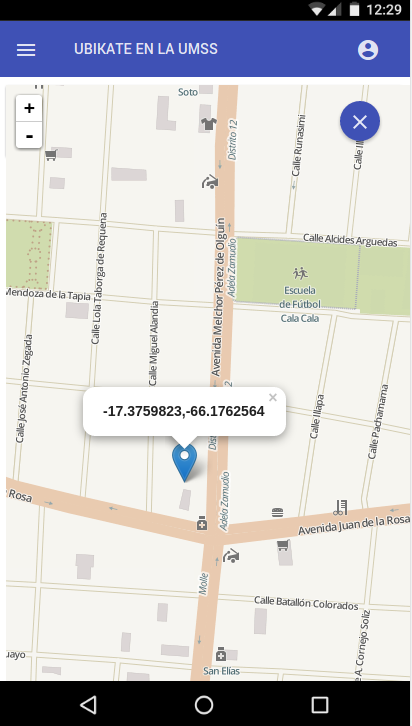
\includegraphics[width=0.5\textwidth]{iteration2/location_marker}
%     \caption*{Fuente: Elaboración propia.}
%   \end{center}
% \end{figure}

\subsubsection{RF018}
\label{subs:RF018}
% Desarrollar un módulo que encuentra la ruta más corta usando la base de datos con información geográfica ruteable de RF012

% Durante esta tarea se investigó la mejor forma de encontrar la ruta más corta y se llegó a la conclusión de usar la combinación de \emph{Postgres + Postgis + pgRouting}, esta investigación se puede apreciar en el marco teórico.\\
%
% Para hallar la ruta más corta se necesita usar las características de la base de datos para poder analizar los datos geográficos almacenados en la Tarea RF012, como el análisis que se requiere hacer es caro osea el costo de procesador para realizar los calculos necesarios es elevado, lo mas recomendable es que este trabajo sea realizado en el backend de la aplicacion por la base de datos.\\
%
% Tambien hay que tomar en cuenta que la tierra no es plana y las líneas que en un mapa parecen lineas rectas, realmente no son rectas, ya que el planeta Tierra es un \emph{esferoide oblato}\footnote{Un \emph{esferoide oblato} (o elipsoide oblato) es un elipsoide de revolución obtenido por rotación de una elipse alrededor de su eje más corto.} por lo que las lineas en apariencia rectas tienen la curvatura natural del planeta Tierra. En distancias largas esto tiene un gran impacto al manejar o utilizar mapas projectados, pero tambien es cierto que para una área pequeña como es el campus de la Universidad de San Simón este problema no tiene un gran impacto pero no está demás en tomar en cuenta esta característica del análisis de datos geoespaciales, como se explico en el capitulo \ref{cha:geolocalizacion}, para el presente proyecto se usara el proyeccion \emph{SRID 3857}.\\

% Una vez que se tienen en cuanta estas variables es necesaria la resolucion del problema de la ruta más corta, \emph{pgRouting} tiene varios métodos implementados para el analisis de datos geo-espaciales en la resolucion de este problema, para el presente proyecto se usara el algoritmo de \emph{Dijkstra}, explicado en el capítulo \ref{cha:ruta_optima}.\\
%
% Tomando en cuenta los conceptos aprendidos y las herramientas investigadas es que se desarrollo el modulo que encuentra la ruta mas corta.

% La siguiente SQL query está diseñado y explicado en la documentación de pgRouting {ref - link}, básicamente se necesita especificar el nodo inicio y el nodo destino y la base de datos se encarga de analizar la tabla creada en RF012, para que el algoritmo de Dijkstra funcione hay que darle un Costo a cada uno de los tramos pertenecientes a la Matriz, en este caso el costo será la longitud del tramo(st_length(geom) AS cost),  el costo de ir del punto A al punto B puede no ser la misma que de ir del punto B al punto A a pesar de ser una única línea, por ejemplo si la circulación fuera en un solo sentido  como en el caso de las rutas para automoviles, en este caso como es una ruta peatonal se simplifica un poco el problema, entonces como datos de entrada tenemos el punto donde se encuentra el usuario extraído por RF017 y el punto del lugar buscado extraído por RF0##, tomando en cuenta estos datos se armó el siguiente query,

% var raw = "SELECT seq, id1 AS node, id2 AS edge, cost " +
%             "FROM pgr_dijkstra('SELECT gid AS id, source::integer, target::integer, st_length(geom) AS cost " +
%             "                   FROM public.ways', " + targetId + ", " + sourceId + ", false, false);";

\subsubsection{RF019}
\label{subs:RF019}
% El usuario puede ver una línea roja que une el marcador de la posición del usuario con el marcador del lugar
% Como resultado de la tarea RF018 se tiene un conjunto de datos en formato de latitud y longitud que conforman líneas, las cuales representan la ruta más corta, pero al final es solo un montón de números, útiles pero para el usuario esta información es difícil de procesar, el usuario necesita información que sea fácil de entender y no existe mejor herramienta disponible para esta tarea que mostrar la \emph{ruta} de forma visual, esto quiere decir que se necesita mostrar la ruta sobre un \emph{mapa}, en la aplicación se usará \emph{ember-leaflet} para desplegar el mapa ofrecido por los servicios de OpenStreetMaps y también para mostrar ruta más corta mediante una línea de color rojo.\\
%
% Para resolver esta tarea se creó un servicio API usando ExpressJS, la cual se encarga obtener la información extraída de la base de datos y transformarla en un objeto JSON (GeoJSON), este objeto contiene la información geoespacial necesaria para ``dibujar'' la línea roja entre 2 puntos georeferenciados, uno de los cuales es el lugar al que se quiere llegar y el otro es la ubicación actual del usuario. \\
%
% \begin{verbatim}
%   ENV.APP.API_HOST + '/api/v1/ways/route/' + sourceData.id + '/' + targetData.id;
%
%   GET /api/v1/ways/route/930/77 200 276.217 ms - 3911
%
%   $ curl http://localhost:3000/api/v1/ways/route/930/77 | python -m json.tool                                                       [3:04:52]
%   % Total    % Received % Xferd  Average Speed   Time    Time     Time  Current
%                                  Dload  Upload   Total   Spent    Left  Speed
% 100  3911  100  3911    0     0   161k      0 --:--:-- --:--:-- --:--:--  166k
% {
%     "features": [
%         {
%             "geometry": {
%                 "coordinates": [
%                     [
%                         -66.1467397848201,
%                         -17.3935321732846
%                     ],
%                     [
%                         -66.1467190789842,
%                         -17.3935294725234
%                     ]
%                 ],
%                 "type": "LineString"
%             },
%             "type": "Feature"
%         },
%
% \end{verbatim}
% % /api/v1/ways/route/
%
% % Este objeto es representado en el mapa usando ember-leaflet con la siguiente instrucción,
% %
% % {{#geojson-layer geoJSON=currentGeoJSON color='red' }}
% % {{/geojson-layer}}
%
% Y se puede observar en el mapa una línea roja que representa la ruta más corta entre el punto donde se encuentra el usuario y el punto del lugar a buscar.
%
% \begin{figure}[H]
%   \begin{center}
%     \caption{Ruta más corta dibujada con una línea roja.}
%     \label{fig:short_way_place}
%     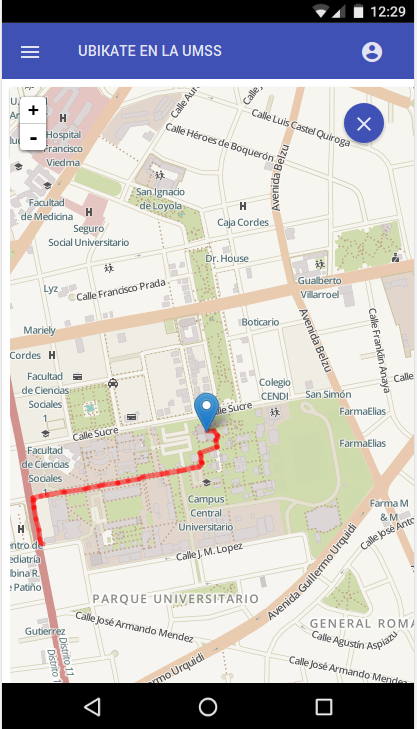
\includegraphics[width=0.5\textwidth]{iteration2/short_way_place}
%     \caption*{Fuente: Elaboración propia.}
%   \end{center}
% \end{figure}

\subsubsection{TS004}
\label{subs:TS004}

Pruebas funcionales

\subsection{Registrar el Avance}
\label{sub:iteracion2_avance}

\subsection{Verificación}
\label{sub:iteracion2_verificacion}


\section{Iteración 3}
\label{sec:iteracion_3}

% Al igual que al principio de la segunda iteración, se esperan los resultados de las pruebas realizadas para poder empezar con la planificación de la tercera iteración.

% \subsection{Iteration Planning Meeting}
% \label{sub:iteration2_planning_meeting}


% Los resultados de las pruebas realizadas se analizan para determinar si los criterios de aceptación, de las historias de usuario trabajadas en la segunda iteración, se cumplen para poder continuar con las historias que continúan sin ser desarrolladas, en caso que las pruebas fallen, es necesario continuar con la implementación de las historias inconclusas.\\
%
% En el caso del presente proyecto, las pruebas pasaron exitosamente y se aceptaron los criterios de aceptación de las historias de usuario trabajadas, por lo tanto se procede con la primera fase del “Iteration Planning”. \\

%
% \subsection{Exploración y Planeación}
% \label{sub:iteration2_exploracion_planeacion}

% Esta fase generalmente se realiza en 2 pasos pero será realizada al mismo tiempo, ya que en la exploración se definen las tareas a realizar y en la planeación se asigna estas tareas al equipo de desarrollo, el cual tiene que estimar las tareas, pero como el equipo de desarrollo está compuesto por mi persona, puedo definir las tareas y asignarles una estimación en el mismo paso.\\
%
% Para la Iteración 3, se trabajarán las historias de usuario 6 y 7, de las que a continuación se definirán sus tareas de ingeniería. \\


\subsection{Planificación de la Iteración 3}

  A continuación se analizará la \emph{historia de usuario} US06, ver el cuadro \ref{tab:US06}.

    
\begin{table}[H]
\begin{center}
  \begin{tabularx}{0.75\textwidth}{ X }
    \toprule
    \textbf{Historia de Usuario:} US06
    \makebox[6cm][r]{\textbf{Prioridad:} Alta} \\
    \makebox[4cm][r]{}
    \makebox[6cm][r]{\textbf{Riesgo:} Alto} \\

    \addlinespace
    \textbf{Nombre:} Añadir más lugares al sistema.\\

    \addlinespace
    \textbf{Descripción:} \\
    \tab Yo como usuario registrado.\\
    \tab Deseo añadir más lugares al sistema. \\
    \tab Para mejorar los criterios de busqueda. \\

    \addlinespace
    \textbf{Criterios de Aceptación:} \\
    \tab Quiero que sea posible anadir un lugar si no lo encuentro en la lista de lugares. \\
    \tab Quiero ver un formulario para poder ingresar los datos de un nuevo lugar.\\
    \tab Quiero pararme cerca o en el lugar que necesito añadir para georeferenciarlo. \\

    \bottomrule
  \end{tabularx}
  \caption{Historia de Usuario - US06}
  \label{tab:US06}
\end{center}
\end{table}


    \begin{table}[H]
  \begin{center}
    \begin{tabularx}{0.75\textwidth}{ X }
      \toprule
      \textbf{Número de Tarea:} T019
      \makebox[1cm][r]{}
      \makebox[6cm][r]{\textbf{Historia de Usuario:} US06} \\

      \addlinespace
      \textbf{Descripción:} Implementar en el backend el \emph{endpoint} para añadir y editar usuarios. \\

      \addlinespace
      \textbf{Tipo de Tarea:} Desarrollo
      \makebox[6cm][r]{\textbf{Estimación [dias]:} 1} \\

      \addlinespace
      \textbf{Programador Responsable:} Edmundo Figueroa \\

      \bottomrule
    \end{tabularx}
    \caption{Tarea de Ingeniería - T019}
    \label{tab:T019}
  \end{center}
\end{table}


\begin{table}[H]
  \begin{center}
    \begin{tabularx}{0.75\textwidth}{ X }
      \toprule
      \textbf{Número de Tarea:} T020
      \makebox[1cm][r]{}
      \makebox[6cm][r]{\textbf{Historia de Usuario:} US06} \\

      \addlinespace
      \textbf{Descripción:} Mostrar un botón para añadir lugares solamente a usuarios registrados. \\

      \addlinespace
      \textbf{Tipo de Tarea:} Desarrollo
      % \makebox[1cm][r]{}
      \makebox[6cm][r]{\textbf{Estimación [dias]:} 0.5} \\

      \addlinespace
      \textbf{Programador Responsable:} Edmundo Figueroa \\

      \bottomrule
    \end{tabularx}
    \caption{Tarea de Ingeniería - T020}
    \label{tab:T020}
  \end{center}
\end{table}

\begin{table}[H]
  \begin{center}
    \begin{tabularx}{0.75\textwidth}{ X }
      \toprule
      \textbf{Número de Tarea:} T021
      \makebox[1cm][r]{}
      \makebox[6cm][r]{\textbf{Historia de Usuario:} US06} \\

      \addlinespace
      \textbf{Descripción:} Mostrar un formulario para añadir más lugares, con el nombre del lugar, descripción, teléfono y nivel. \\

      \addlinespace
      \textbf{Tipo de Tarea:} Desarrollo
      \makebox[6cm][r]{\textbf{Estimación [dias]:} 0.5} \\

      \addlinespace
      \textbf{Programador Responsable:} Edmundo Figueroa \\

      \bottomrule
    \end{tabularx}
    \caption{Tarea de Ingeniería - T021}
    \label{tab:T021}
  \end{center}
\end{table}

\begin{table}[H]
  \begin{center}
    \begin{tabularx}{0.75\textwidth}{ X }
      \toprule
      \textbf{Número de Tarea:} T022
      \makebox[1cm][r]{}
      \makebox[6cm][r]{\textbf{Historia de Usuario:} US06} \\

      \addlinespace
      \textbf{Descripción:} Registrar las coordenadas del lugar al momento de crear un nuevo lugar. \\

      \addlinespace
      \textbf{Tipo de Tarea:} Desarrollo
      \makebox[6cm][r]{\textbf{Estimación [dias]:} 1} \\

      \addlinespace
      \textbf{Programador Responsable:} Edmundo Figueroa \\

      \bottomrule
    \end{tabularx}
    \caption{Tarea de Ingeniería - T022}
    \label{tab:T022}
  \end{center}
\end{table}


\begin{table}[H]
  \begin{center}
    \begin{tabularx}{0.75\textwidth}{ X }
      \toprule
      \textbf{Número de Tarea:} T023
      \makebox[1cm][r]{}
      \makebox[6cm][r]{\textbf{Historia de Usuario:} US06} \\

      \addlinespace
      \textbf{Descripción:} Implementar el modulo para poder agregar una foto a un lugar. \\

      \addlinespace
      \textbf{Tipo de Tarea:} Desarrollo
      \makebox[6cm][r]{\textbf{Estimación [dias]:} 1} \\

      \addlinespace
      \textbf{Programador Responsable:} Edmundo Figueroa \\

      \bottomrule
    \end{tabularx}
    \caption{Tarea de Ingeniería - T023}
    \label{tab:T023}
  \end{center}
\end{table}


  A continuación se analizará la \emph{historia de usuario} US07, ver el cuadro \ref{tab:US07}.

    
\begin{table}[H]
\begin{center}
 \begin{tabularx}{0.75\textwidth}{ X }
   \toprule
   \textbf{Historia de Usuario:} US07
   \makebox[6cm][r]{\textbf{Prioridad:} Alta} \\
   \makebox[4cm][r]{}
   \makebox[6cm][r]{\textbf{Riesgo:} Alto} \\

   \addlinespace
   \textbf{Nombre:} Editar la información de un lugar.\\

   \addlinespace
   \textbf{Descripción:} \\
   \tab Yo como usuario registrado.\\
   \tab Deseo editar la información de un lugar. \\
   \tab Para mejorar o corregir la información de ese lugar. \\

   \addlinespace
   \textbf{Criterios de Aceptación:} \\
   \tab Al entrar a la información de un lugar quiero ser el único que vea un icono para poder entrar a la edición de los datos. \\
   \tab Quiero acceder a un formulario que muestre la información actual del lugar y poder editar la información mostrada. \\

   \bottomrule
 \end{tabularx}
 \caption{Historia de Usuario - US07}
 \label{tab:US07}
\end{center}
\end{table}


    \begin{table}[H]
  \begin{center}
    \begin{tabularx}{0.75\textwidth}{ X }
      \toprule
      \textbf{Número de Tarea:} T024
      \makebox[1cm][r]{}
      \makebox[6cm][r]{\textbf{Historia de Usuario:} US07} \\

      \addlinespace
      \textbf{Descripción:} Implementar el modulo para editar lugares. \\

      \addlinespace
      \textbf{Tipo de Tarea:} Desarrollo
      \makebox[6cm][r]{\textbf{Estimación [dias]:} 1} \\

      \addlinespace
      \textbf{Programador Responsable:} Edmundo Figueroa \\

      \bottomrule
    \end{tabularx}
    \caption{Tarea de Ingeniería - T024}
    \label{tab:T024}
  \end{center}
\end{table}


\begin{table}[H]
  \begin{center}
    \begin{tabularx}{0.75\textwidth}{ X }
      \toprule
      \textbf{Número de Tarea:} T025
      \makebox[1cm][r]{}
      \makebox[6cm][r]{\textbf{Historia de Usuario:} US07} \\

      \addlinespace
      \textbf{Descripción:} Mostrar un botón para editar un lugar solamente a usuarios administradores. \\

      \addlinespace
      \textbf{Tipo de Tarea:} Desarrollo
      % \makebox[1cm][r]{}
      \makebox[6cm][r]{\textbf{Estimación [dias]:} 0.5} \\

      \addlinespace
      \textbf{Programador Responsable:} Edmundo Figueroa \\

      \bottomrule
    \end{tabularx}
    \caption{Tarea de Ingeniería - T025}
    \label{tab:T025}
  \end{center}
\end{table}

\begin{table}[H]
  \begin{center}
    \begin{tabularx}{0.75\textwidth}{ X }
      \toprule
      \textbf{Número de Tarea:} T026
      \makebox[1cm][r]{}
      \makebox[6cm][r]{\textbf{Historia de Usuario:} US07} \\

      \addlinespace
      \textbf{Descripción:} Mostrar la información actual del lugar en el formalario de edicion. \\

      \addlinespace
      \textbf{Tipo de Tarea:} Desarrollo
      \makebox[6cm][r]{\textbf{Estimación [dias]:} 0.5} \\

      \addlinespace
      \textbf{Programador Responsable:} Edmundo Figueroa \\

      \bottomrule
    \end{tabularx}
    \caption{Tarea de Ingeniería - T026}
    \label{tab:T026}
  \end{center}
\end{table}

\begin{table}[H]
  \begin{center}
    \begin{tabularx}{0.75\textwidth}{ X }
      \toprule
      \textbf{Número de Tarea:} T027
      \makebox[1cm][r]{}
      \makebox[6cm][r]{\textbf{Historia de Usuario:} US07} \\

      \addlinespace
      \textbf{Descripción:} Mostrar un boton para eliminar el lugar solamente a un usuario administrador. \\

      \addlinespace
      \textbf{Tipo de Tarea:} Desarrollo
      \makebox[6cm][r]{\textbf{Estimación [dias]:} 1} \\

      \addlinespace
      \textbf{Programador Responsable:} Edmundo Figueroa \\

      \bottomrule
    \end{tabularx}
    \caption{Tarea de Ingeniería - T027}
    \label{tab:T027}
  \end{center}
\end{table}



% \subsubsection{Tareas del US06}
% \label{sub:us06_tasks}

% \begin{table}[H]
  \begin{center}
    \begin{tabularx}{\textwidth}{ c  X  C{2.3cm} }
      \toprule
        \textbf{Código} &
        \multicolumn{1}{c}{\textbf{Tarea}} &
        \textbf{Estimación [dias]}\\

      \midrule
        T020
        &
        El usuario podrá ver un link hacia el formulario para añadir más lugares desde la lista de lugares existentes.
        &
        0.5 \\

      \addlinespace
        T021
        &
        El usuario podrá ver un formulario para añadir un lugar con información básica. por ejemplo, el nombre del lugar, descripción, teléfono.
        &
        1 \\

      \addlinespace
        T022
        &
        El usuario deberá estar cerca del lugar que desea añadir para poder georeferenciarlo.
        &
        1 \\

      \addlinespace
        T023
        &
        Un usuario no-administrador no debería poder ver el formulario para añadir lugares.
        &
        1 \\


      \addlinespace
        P004
        &
        Crear pruebas de funcionalidad del US05.
        &
        0.5 \\

      \addlinespace
      \midrule
        & \multicolumn{1}{R{7cm}}{\textbf{Total: }}
        & 4 \\

      \bottomrule
    \end{tabularx}
    \caption{Tareas del US05}
    \label{tab:us05_tasks}
  \end{center}
\end{table}

%
%
% \subsubsection{Tareas del US07}
% \label{sub:us07_tasks}

  % \begin{table}[H]
  \begin{center}
    \begin{tabularx}{\textwidth}{ c  X  C{2.3cm} }
      \toprule
        \textbf{Código} &
        \multicolumn{1}{c}{\textbf{Tarea}} &
        \textbf{Estimación [dias]}\\

      \midrule
      T024
      &
      Implementar en el backend el \emph{endpoint} para eliminar usuarios.
      &
      0.5 \\

      \addlinespace
        T024
        &
        Mostrar un boton solamente al administrador para editar un lugar.
        &
        0.5 \\

      \addlinespace
        T025
        &
        Mostrar la información actual del lugar en el formalario de edicion
        % El usuario debería poder ver la información actual del lugar en el formulario para editar el lugar.
        &
        1 \\

      \addlinespace
        T026
        &
        Mostrar un boton para eliminar el lugar solamente a un usuario administrador.
        % El usuario no-administrador no debería poder ver el link hacia el formulario para editar el lugar.
        &
        1 \\

      \addlinespace
        P005
        &
        Crear pruebas de funcionalidad del US06.
        &
        0.5 \\

      \addlinespace
      \midrule
        & \multicolumn{1}{R{7cm}}{\textbf{Total: }}
        & 3 \\

      \bottomrule
    \end{tabularx}
    \caption{Tareas del US06}
    \label{tab:us06_tasks}
  \end{center}
\end{table}



  % \subsection{Implementación}
  % \label{sub:implementacion_iteracion_3}

  \subsection{Implementación de la Iteración 3}


      
% \subsubsection{Implementar módulo para añadir lugares al sistema}
\subsubsection{Registro de Lugares en el sistema}

Para registrar un \emph{lugar} primeramente se implementó el formulario que se usará para recolectar la información del \emph{lugar}, el formulario fue creado usando \emph{EmberJs} y se lo puede ver en la figura \ref{fig:new_place}. \\

\begin{figure}[H]
     \begin{center}
       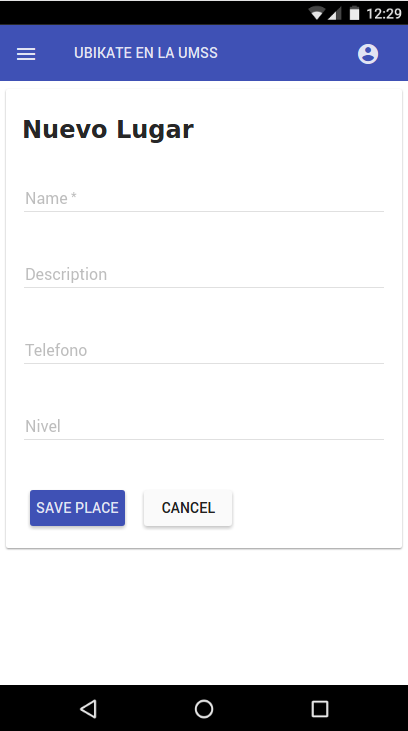
\includegraphics[width=0.3\textwidth]{new_place}

       \caption{Formulario para añadir un nuevo \emph{lugar}.}
       \label{fig:new_place}
       \caption*{Fuente: Elaboración propia.}
     \end{center}
\end{figure}

Posteriormente es necesario crear la petición HTTP desde el controlador de \emph{EmberJS} hacia el API, en el cuerpo de la petición se incluye la posición georeferenciada del celular utilizando el API de Geolocalización de HTML5 usada anteriormente para encontrar la ubicación del usuario, también se incluye el nombre, la descripción, el teléfono y el nivel del \emph{lugar}. En el codigo \ref{new_place_request} se puede ver la implementación de la petición.


% En la figura \ref{fig:new_place} se puede ver el formulario implementado usando \emph{ember-paper}, el cual colecciona los datos que se quieren introducir y se los envía al backend usando una llamada AJAX, como se puede ver en el siguiente código, para crear la petición POST se obtiene las coordenadas actuales del dispositivo móvil además de los datos recolectados del formulario y que con la ayuda de \emph{JQuery} es enviado al API el cual maneja la información recibida y se encarga de insertar los datos en la base de datos.\\

% \newpage
\begin{center}
 \begin{lstlisting}[label=new_place_request,caption=POST request creado en el controlador de \emph{ember}]

   var payload = {
       name: nombre,
       description: descripcion,
       phone: telefono,
       level: nivel,
       lat: latitud,
       lon: longitud
   };

   var url = (ENV.APP.API_HOST || '') + '/api/v1/places/';
   jQuery.post(url, payload).then(
       function(data) {
           var transition = controller.get('transition');
           if (transition) {
               self.transitionTo('places.show');
           } else {
               self.transitionTo('places');
           }
       },
       function(error) {
           controller.set('message', error.responseText);
       }
   );

 \end{lstlisting}
\end{center}

% En esta iteración se implementó la opción de añadir más lugares al sistema, de editarlos y eliminarlos, y la primera tarea es crear las consultas SQL para llevar a cabo las tareas. \\

% por lo que es necesario crear las consultas SQL que insertaran los datos enviados desde el dispositivo móvil al servidor. \\

% Como requisito para insertar un nuevo ``lugar'', se requiere que el usuario esté posicionado en el ``lugar'' ya que se usaran sus coordenadas para posicionar el ``lugar''. Las coordenadas del usuario son obtenidas usando el API de Geolocalización propia de HTML5, usada anteriormente para encontrar la ubicación del usuario \emph{visitante} en la iteración 2.\\

% Posteriormente se necesita implementar el formulario que el usuario usará para insertar los datos del ``lugar'': el nombre, la descripción, el teléfono y el nivel.\\

% Para insertar un ``lugar''  en la base de datos se usó el codigo \ref{new_place}, donde se puede observar la consulta SQL usada, para la cual se necesita capturar la latitud y longitud respectiva donde se encuentra el usuario, además de los datos del ``lugar''.\\

La petición creada es recibida en el API utilizando el \emph{endpoint} RESTful designado para ello, \verb|router.post('/', places.newPlace);|, el \emph{endpoint} se encarga de mandar la información recibida hacia la base de de datos, tomando en cuenta que la posición del lugar es un tipo especial de la base de datos, la latitud y longitud necesitan ser transformadas al momento de insertar el \emph{lugar} en la base de datos, como se muestra en el codigo \ref{cod-new_place_api}.


\begin{center}
 \begin{lstlisting}[label=cod-new_place_api,caption=Insertar un ``lugar'' en la base de datos.]

   router.post('/', places.newPlace);

   var newPlace = (req, res) => {
       var name = req.body.name || '';
       var lat = req.body.lat || '';
       var lon = req.body.lon || '';
       var description = req.body.description || '';
       var phone = req.body.phone || '';
       var level = req.body.level || '';

       let raw = `insert into place (name, geom, description, phone, level)
                  values ('${name}',
                          ST_GeomFromText('POINT(${lon} ${lat})', 3875),
                          '${description}',
                          '${phone}',
                          '${level}'
                         );`;

       Knex.raw(raw)
           .then(function(data) {
               res.json({
                   "message": "Place saved successfully!",
                   "data": data
               });
           })
           .catch(function(error) {
               res.send("Error:", error);
           });
   };

 \end{lstlisting}
\end{center}




% Para la creación de un ``lugar'' es necesario implementar un \emph{endpoint} en el API y siguiendo las convenciones REST se , para que como ya se explicó anteriormente el frontend pueda comunicarse con el backend. \\

% En el API de la aplicación, se implementó un \emph{endpoint} para que pueda manejar los \emph{request} del cliente para añadir un lugar, este \emph{request} es enviado usando el verbo HTTP \emph{POST}, que como ya se explicó es el usado en un REST API para crear objetos. \\

\subsubsection{Edición de la información del Lugar}

Para editar de la información de un lugar se rehusó el formulario ya creado para el registro del mismo, pero populando los campos con la información actual del lugar, el resultado se lo puede ver en la figura \ref{fig:place_edit_form}. \\

\begin{figure}[H]
     \begin{center}
       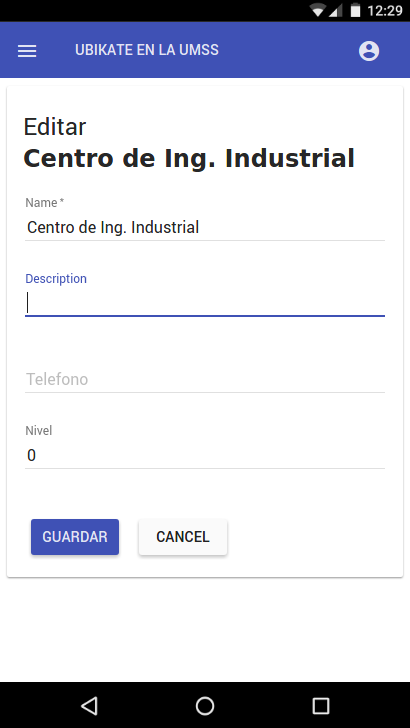
\includegraphics[width=0.3\textwidth]{place_edit_form}

       \caption{Formulario para editar un \emph{lugar}}
       \label{fig:place_edit_form}
       \caption*{Fuente: Elaboración propia.}
     \end{center}
\end{figure}


Los cambios a la información del \emph{lugar} son enviados al API mediante una petición PUT, siguiendo los lineamientos del REST API implementado, esta petición se puede ver en el codigo \ref{cod-edit_place_request}.

% \newpage
\begin{center}
 \begin{lstlisting}[label=cod-edit_place_request,caption=Petición HTTP para editar un lugar.]

   router.put('/:id', places.editPlace);

   var body = {
       name: name,
       description: description,
       phone: phone,
       level: level
   };

   var url = (ENV.APP.API_HOST || '') + `/api/v1/places/${id}`;
   jQuery.ajax({
       url: url,
       type: 'put',
       data: body
   }).then(
       function(data) {
           self.transitionTo('places.show', id);
       },
       function(error) {
           controller.set('message', error.responseText);
       }
   );

 \end{lstlisting}
\end{center}

A diferencia del registro del \emph{lugar}, que guarda la posición georeferenciada al momento de registrar el \emph{lugar}, en la edición de los datos no se está tomando en cuenta este dato porque se noto que generalmente cuando se requiere actualizar los datos del \emph{lugar}, el usuario no se encuentra en la posición original del \emph{lugar} y este dato se pierde, corrompiendo la base de datos. Es por esta razón que se decidió que no se actualizará la posición geográfica del \emph{lugar} sin alguna opción explícita que advierta al usuario de las consecuencias de esta acción, pero como tal tarea no se halla dentro de la \emph{historia de usuario} que se esta implementado, se tomo la decisión de realizarla en una futura iteración.








% \subsubsection{Eliminar un lugar}

% Una vez implementado la lógica para añadir un ``lugar'', se implementó los módulos para poder eliminar el ``lugar'', para esto se añadió un botón en la lista de lugares, el cual despliega un mensaje de advertencia al usuario de que está por eliminar un ``lugar'' y que la acción es irreversible, por lo tanto este botón sólo está disponible para un usuario \emph{administrador}. \\
%
% La verbo  HTTP \emph{DELETE} es el que de acuerdo a la implementación del API REST es el adecuado para eliminar un lugar, por lo tanto es el que se usó en la aplicación. En el codigo \ref{delete_place_enpoint} se puede observar el \emph{endpoint} implementado en el API que se encarga de manejar las peticiones \emph{DELETE} creando una consulta SQL que elimina el lugar de la base de datos.\\
%
% \begin{center}
%   \begin{lstlisting}[label=delete_place_enpoint,caption=DELETE request elimina un lugar.]
%
%     router.delete('/:id', places.deletePlace);
%
%     var deletePlace = (req, res) => {
%         var id = req.params.id;
%
%         Place.forge({
%             gid: id
%         })
%         .destroy()
%         .then(function(model) {
%             res.json({
%                 "message": "Place deleted successfully!"
%             });
%         })
%         .catch(function(err) {
%             res.status(500);
%         });
%     };
%
%   \end{lstlisting}
% \end{center}
%
% En el anterior codigo se puede apreciar la bondad de usar un manejador de bases de datos como \emph{Bookshelf} ya que usando el método \verb|destroy()|, se encarga automáticamente de crear la consulta SQL para eliminar una tupla de la base de datos.\\


  \subsection{Pruebas de Aceptación de la Iteración 3}

      \begin{table}[H]
  \begin{center}
    \begin{tabularx}{0.75\textwidth}{ X }
      \toprule
      \textbf{Codigo:} CP012
      \makebox[3cm][r]{}
      \makebox[6cm][r]{\textbf{Historia de Usuario:} US06} \\

      \addlinespace
      \textbf{Tipo:} Prueba de Funcionalidad - Positiva. \\

      \addlinespace
      \textbf{Nombre:} Verificar el registro de lugares. \\

      \addlinespace
      \textbf{Descripción:} Validar que un usuario registrado puede añadir un lugar nuevo al sistema. \\

      \addlinespace
      \textbf{Condiciones de Ejecución:} \\
      \tab \textbf{a.} El usuario debe estar registrado. \\
      % \tab \textbf{b.} Registrar un lugar dentro del campus Universitario.\\

      \addlinespace
      \textbf{Entradas / Pasos de Ejecución:}  \\
      \tab \textbf{1.} Seleccionar el menú \emph{Lugares}. \\
      \tab \textbf{2.} Hacer tap sobre el icono de registro de lugares.\\
      \tab \textbf{3.} Ingresar el Nombre del lugar.\\
      \tab \textbf{4.} Ingresar una Descripción del lugar.\\
      \tab \textbf{5.} Ingresar el Teléfono del lugar.\\
      \tab \textbf{6.} Ingresar el Nivel del lugar.\\
      \tab \textbf{7.} Aceptar el formulario.\\


      \addlinespace
      \textbf{Resultado Esperado:} Una vista de la información del lugar es desplegada con los datos ingresados en los pasos.  \\

      \addlinespace
      \textbf{Evaluación de la Prueba:} Prueba exitosa. \\

      \bottomrule
    \end{tabularx}
    \caption{Prueba de Aceptación - CP012}
    \label{tab:CP012}
  \end{center}
\end{table}

\begin{table}[H]
  \begin{center}
    \begin{tabularx}{0.75\textwidth}{ X }
      \toprule
      \textbf{Codigo:} CP013
      \makebox[3cm][r]{}
      \makebox[6cm][r]{\textbf{Historia de Usuario:} US07} \\

      \addlinespace
      \textbf{Tipo:} Prueba de Funcionalidad - Positiva. \\

      \addlinespace
      \textbf{Nombre:} Verificar la edición de la información de un lugar. \\

      \addlinespace
      \textbf{Descripción:} Validar que un usuario registrado puede editar la información de un lugar. \\

      \addlinespace
      \textbf{Condiciones de Ejecución:} \\
      \tab \textbf{a.} El usuario debe estar registrado. \\
      \tab \textbf{b.} Registrar un lugar dentro del campus Universitario.\\

      \addlinespace
      \textbf{Entradas / Pasos de Ejecución:}  \\
      \tab \textbf{1.} Seleccionar el menú \emph{Lugares}. \\
      \tab \textbf{2.} Buscar el lugar registrado en las condiciones.\\
      \tab \textbf{3.} Editar el Nombre del lugar.\\
      \tab \textbf{4.} Editar la Descripción del lugar.\\
      \tab \textbf{5.} Editar el Teléfono del lugar.\\
      \tab \textbf{6.} Editar el Nivel del lugar.\\
      \tab \textbf{7.} Aceptar el formulario.\\


      \addlinespace
      \textbf{Resultado Esperado:} Una vista de la información del lugar es desplegada con la información editada en los pasos.  \\

      \addlinespace
      \textbf{Evaluación de la Prueba:} Prueba exitosa. \\

      \bottomrule
    \end{tabularx}
    \caption{Prueba de Aceptación - CP013}
    \label{tab:CP013}
  \end{center}
\end{table}


\begin{table}[H]
  \begin{center}
    \begin{tabularx}{0.75\textwidth}{ X }
      \toprule
      \textbf{Codigo:} CP014
      \makebox[3cm][r]{}
      \makebox[6cm][r]{\textbf{Historia de Usuario:} US06} \\

      \addlinespace
      \textbf{Tipo:} Prueba de Funcionalidad - Negativa. \\

      \addlinespace
      \textbf{Nombre:} Verificar que no pueda registrar un lugar fuera del campus Universitario. \\

      \addlinespace
      \textbf{Descripción:} Validar que los lugares que están fuera del campus Universitario no pueda ser registrado en el sistema. \\

      \addlinespace
      \textbf{Condiciones de Ejecución:} \\
      \tab \textbf{a.} El usuario debe estar registrado. \\
      \tab \textbf{b.} El usuario debe estar fuera de los predios del Campus Universitario.\\

      \addlinespace
      \textbf{Entradas / Pasos de Ejecución:}  \\
      \tab \textbf{1.} Seleccionar el menú \emph{Lugares}. \\
      \tab \textbf{2.} Hacer tap sobre el icono de registro de lugares.\\

      \addlinespace
      \textbf{Resultado Esperado:} Un mensaje debería ser desplegado informando que no se pueden registrar Lugares fuera del Campus Universitario.  \\

      \addlinespace
      \textbf{Evaluación de la Prueba:} Prueba fallada. \\

      \bottomrule
    \end{tabularx}
    \caption{Prueba de Aceptación - CP014}
    \label{tab:CP014}
  \end{center}
\end{table}


\begin{table}[H]
  \begin{center}
    \begin{tabularx}{0.75\textwidth}{ X }
      \toprule
      \textbf{Codigo:} CP015
      \makebox[3cm][r]{}
      \makebox[6cm][r]{\textbf{Historia de Usuario:} US06, US07} \\

      \addlinespace
      \textbf{Tipo:} Prueba de Usabilidad. \\

      \addlinespace
      \textbf{Nombre:} Verificar los campos de texto de los formularios de registro y edición. \\

      \addlinespace
      \textbf{Descripción:} Validar que los campos de texto dentro los formularios de registro y edición de lugares no exceda la longitud de la pantalla del dispositivo móvil. \\

      \addlinespace
      \textbf{Condiciones de Ejecución:} \\
      \tab \textbf{a.} El usuario debe estar registrado. \\
      % \tab \textbf{b.} El usuario debe estar fuera de los predios del Campus Universitario.\\

      \addlinespace
      \textbf{Entradas / Pasos de Ejecución:}  \\
      \tab \textbf{1.} Seleccionar el menú \emph{Lugares}. \\
      \tab \textbf{2.} Presionar el icono de registro de lugares.\\
      \tab \textbf{3.} Insertar texto en los campos de descripción, teléfono y nombre.\\
      \tab \textbf{4.} Repetir para el formulario de edición de lugares.\\

      \addlinespace
      \textbf{Resultado Esperado:} El texto escrito no debería sobrepasar la longitud del dispositivo móvil en los formularios de registro y edición de lugares.  \\

      \addlinespace
      \textbf{Evaluación de la Prueba:} Prueba exitosa. \\

      \bottomrule
    \end{tabularx}
    \caption{Prueba de Aceptación - CP015}
    \label{tab:CP015}
  \end{center}
\end{table}


  % \subsection{Registrar el Avance}
  % \label{sub:iteracion3_avance}

  % \subsection{Verificación}
  % \label{sub:iteracion3_verificacion}


\section{Iteración 3}
\label{sec:iteracion_3}

Al igual que al principio de la segunda iteración, se esperan los resultados de las pruebas realizadas para poder empezar con la planificación de la tercera iteración.

\subsection{Iteration Planning Meeting}
\label{sub:iteration2_planning_meeting}


Los resultados de las pruebas realizadas se analizan para determinar si los criterios de aceptación, de las historias de usuario trabajadas en la segunda iteración, se cumplen para poder continuar con las historias que continúan sin ser desarrolladas, en caso que las pruebas fallen, es necesario continuar con la implementación de las historias inconclusas.\\

En el caso del presente proyecto, las pruebas pasaron exitosamente y se aceptaron los criterios de aceptación de las historias de usuario trabajadas, por lo tanto se procede con la primera fase del “Iteration Planning”. \\


\subsection{Exploración y Planeación}
\label{sub:iteration2_exploracion_planeacion}

Esta fase generalmente se realiza en 2 pasos pero será realizada al mismo tiempo, ya que en la exploración se definen las tareas a realizar y en la planeación se asigna estas tareas al equipo de desarrollo, el cual tiene que estimar las tareas, pero como el equipo de desarrollo está compuesto por mi persona, puedo definir las tareas y asignarles una estimación en el mismo paso.\\

Para la Iteración 3, se trabajarán las historias de usuario 5 y 6, de las cuales serán definidas sus tareas de desarrollo en las siguientes tablas.


\subsection{Tareas del US05}
\label{sub:us05_tasks}

  \begin{table}[H]
  \begin{center}
    \begin{tabularx}{\textwidth}{ c  X  C{2.3cm} }
      \toprule
        \textbf{Código} &
        \multicolumn{1}{c}{\textbf{Tarea}} &
        \textbf{Estimación [dias]}\\

      \midrule
        RF020
        &
        El usuario podrá ver un link hacia el formulario para añadir más lugares desde la lista de lugares existentes.
        &
        0.5 \\

      \addlinespace
        RF021
        &
        El usuario podrá ver un formulario para añadir un lugar con información básica. por ejemplo, el nombre del lugar, descripción, teléfono.
        &
        1 \\

      \addlinespace
        RF022
        &
        El usuario deberá estar cerca del lugar que desea añadir para poder georeferenciarlo.
        &
        1 \\

      \addlinespace
        RF023
        &
        Un usuario no-administrador no debería poder ver el formulario para añadir lugares.
        &
        1 \\


      \addlinespace
        TS004
        &
        Crear pruebas de funcionalidad del US05.
        &
        0.5 \\

      \addlinespace
      \midrule
        & \multicolumn{1}{R{7cm}}{\textbf{Total: }}
        & 4 \\

      \bottomrule
    \end{tabularx}
    \caption{Tareas del US05}
    \label{tab:us05_tasks}
  \end{center}
\end{table}


\subsection{Tareas del US06}
\label{sub:us06_tasks}

  \begin{table}[H]
  \begin{center}
    \begin{tabularx}{\textwidth}{ c  X  C{2.3cm} }
      \toprule
        \textbf{Código} &
        \multicolumn{1}{c}{\textbf{Tarea}} &
        \textbf{Estimación [dias]}\\

      \midrule
        T020
        &
        El usuario podrá ver un link hacia el formulario para añadir más lugares desde la lista de lugares existentes.
        &
        0.5 \\

      \addlinespace
        T021
        &
        El usuario podrá ver un formulario para añadir un lugar con información básica. por ejemplo, el nombre del lugar, descripción, teléfono.
        &
        1 \\

      \addlinespace
        T022
        &
        El usuario deberá estar cerca del lugar que desea añadir para poder georeferenciarlo.
        &
        1 \\

      \addlinespace
        T023
        &
        Un usuario no-administrador no debería poder ver el formulario para añadir lugares.
        &
        1 \\


      \addlinespace
        P004
        &
        Crear pruebas de funcionalidad del US05.
        &
        0.5 \\

      \addlinespace
      \midrule
        & \multicolumn{1}{R{7cm}}{\textbf{Total: }}
        & 4 \\

      \bottomrule
    \end{tabularx}
    \caption{Tareas del US05}
    \label{tab:us05_tasks}
  \end{center}
\end{table}




% end desarrollo
